\documentclass[a4paper]{article}
\usepackage{lmodern}
\usepackage{amssymb,amsmath}
\usepackage{ifxetex,ifluatex}
\usepackage{fixltx2e} % provides \textsubscript
\ifnum 0\ifxetex 1\fi\ifluatex 1\fi=0 % if pdftex
  \usepackage[T1]{fontenc}
  \usepackage[utf8]{inputenc}
\else % if luatex or xelatex
  \ifxetex
    \usepackage{mathspec}
  \else
    \usepackage{fontspec}
  \fi
  \defaultfontfeatures{Ligatures=TeX,Scale=MatchLowercase}
\fi
% use upquote if available, for straight quotes in verbatim environments
\IfFileExists{upquote.sty}{\usepackage{upquote}}{}
% use microtype if available
\IfFileExists{microtype.sty}{%
\usepackage{microtype}
\UseMicrotypeSet[protrusion]{basicmath} % disable protrusion for tt fonts
}{}
\usepackage[margin=1in]{geometry}
\usepackage{hyperref}
\hypersetup{unicode=true,
            pdftitle={Distribuição Log-Normal},
            pdfauthor={Luiz Fernando Palin Droubi; Norberto Hochheim; Willian Zonato},
            pdfborder={0 0 0},
            breaklinks=true}
\urlstyle{same}  % don't use monospace font for urls
\usepackage{graphicx,grffile}
\makeatletter
\def\maxwidth{\ifdim\Gin@nat@width>\linewidth\linewidth\else\Gin@nat@width\fi}
\def\maxheight{\ifdim\Gin@nat@height>\textheight\textheight\else\Gin@nat@height\fi}
\makeatother
% Scale images if necessary, so that they will not overflow the page
% margins by default, and it is still possible to overwrite the defaults
% using explicit options in \includegraphics[width, height, ...]{}
\setkeys{Gin}{width=\maxwidth,height=\maxheight,keepaspectratio}
\IfFileExists{parskip.sty}{%
\usepackage{parskip}
}{% else
\setlength{\parindent}{0pt}
\setlength{\parskip}{6pt plus 2pt minus 1pt}
}
\setlength{\emergencystretch}{3em}  % prevent overfull lines
\providecommand{\tightlist}{%
  \setlength{\itemsep}{0pt}\setlength{\parskip}{0pt}}
\setcounter{secnumdepth}{5}
% Redefines (sub)paragraphs to behave more like sections
\ifx\paragraph\undefined\else
\let\oldparagraph\paragraph
\renewcommand{\paragraph}[1]{\oldparagraph{#1}\mbox{}}
\fi
\ifx\subparagraph\undefined\else
\let\oldsubparagraph\subparagraph
\renewcommand{\subparagraph}[1]{\oldsubparagraph{#1}\mbox{}}
\fi

%%% Use protect on footnotes to avoid problems with footnotes in titles
\let\rmarkdownfootnote\footnote%
\def\footnote{\protect\rmarkdownfootnote}

%%% Change title format to be more compact
\usepackage{titling}

% Create subtitle command for use in maketitle
\newcommand{\subtitle}[1]{
  \posttitle{
    \begin{center}\large#1\end{center}
    }
}

\setlength{\droptitle}{-2em}
  \title{Distribuição Log-Normal}
  \pretitle{\vspace{\droptitle}\centering\huge}
  \posttitle{\par}
\subtitle{Propriedades e aplicações}
  \author{Luiz Fernando Palin Droubi\footnote{SPU/SC,
  \href{mailto:luiz.droubi@planejamento.gov.br}{\nolinkurl{luiz.droubi@planejamento.gov.br}}} \\ Norberto Hochheim\footnote{UFSC,
  \href{mailto:hochheim@gmail.com}{\nolinkurl{hochheim@gmail.com}}} \\ Willian Zonato\footnote{SPU/SC,
  \href{mailto:willian.zonato@planejamento.gov.br}{\nolinkurl{willian.zonato@planejamento.gov.br}}}}
  \preauthor{\centering\large\emph}
  \postauthor{\par}
  \predate{\centering\large\emph}
  \postdate{\par}
  \date{13/06/2018}

\usepackage[brazil]{babel}
\usepackage{graphicx}
\usepackage{float}
\usepackage{subfig}
\usepackage{caption}
\newcommand{\pkg}[1]{{\normalfont\fontseries{b}\selectfont #1}}
\let\proglang=\textsf
\let\code=\texttt
\usepackage{booktabs}
\usepackage{longtable}
\usepackage{array}
\usepackage{multirow}
\usepackage[table]{xcolor}
\usepackage{wrapfig}
\usepackage{float}
\usepackage{colortbl}
\usepackage{pdflscape}
\usepackage{tabu}
\usepackage{threeparttable}
\usepackage[normalem]{ulem}

\usepackage{amsmath,amssymb}

\begin{document}
\maketitle

\section{INTRODUÇÃO}\label{introducao}

A transformação de variáveis é um procedimento comum na Engenharia de
Avaliações. No entanto, a transformação dos dados por vezes é realizada
sem uma análise profunda do comportamento das variáveis. A \emph{Food
and Drug Administration} (FDA), órgão federal dos EUA que atua no
controle da comercialização de alimentos e medicamentos no país,
recomenda:

\begin{quote}
A transformação desnecessária de dados deve ser evitada. Caso tenha sido
realizada transformação de dados, uma justificativa para a escolha da
transformação junto com a interpretação das estimativas dos efeitos do
tratamento com base nos dados transformados deve ser fornecida.(FDA,
\protect\hyperlink{ref-fda}{1988} apud KEENE
(\protect\hyperlink{ref-keene}{1985}))
\end{quote}

No entanto, a transformação logarítmica é especial, por uma série de
aspectos, como pode ser visto em KEENE
(\protect\hyperlink{ref-keene}{1985}).

A distribuição lognormal apresenta diversas aplicações práticas. É
comum, na área de avaliação de imóveis, mas não apenas\footnote{Dados
  estritamente positivos, como valores em moeda, altura, peso, etc,
  normalmente seguem a distribuição lognormal.}, nos depararmos com
dados que seguem esta distribuição. Neste artigo pretendemos demonstrar
as principais características da distribuição lognormal, sua relação com
a distribuição normal de Gauss, assim como debatemos a melhor maneira de
se lidar com dados lognormais.

\section{REVISÃO BIBLIOGRÁFICA}\label{revisao-bibliografica}

\subsection{Formulação}\label{formulacao}

A formulação da distribuição lognormal para os parâmetros \(\mu\) e
\(\sigma\) pode ser vista abaixo (ACTION)

\[\begin{cases}
f(x;\mu, \sigma) = \frac{1}{x\sigma\sqrt{2\pi}}\exp(-\frac{(log(x) - \mu)^2}{2\sigma^2}) & \forall x > 0 \\ 
0 & \text{ se } x = 0 
\end{cases}\]

\subsection{Propriedades}\label{propriedades}

\subsubsection{Valor Esperado e
Variância}\label{valor-esperado-e-variancia}

O valor Esperado \(\mathbb{E}\) de uma variável aleatória com
distribuição lognormal \(X\) é (ACTION):

\[\mathbb{E}(X) = \exp \left (\mu + \frac{\sigma^2}{2} \right )\] E sua
variância é:

\[\newcommand{\Var}{\operatorname{Var}} \Var(X) = \exp (2\mu+\sigma^2)(\exp(\sigma^2)-1)\]

\subsubsection{Medidas de Tendência
Central}\label{medidas-de-tendencia-central}

A figura \ref{fig:densidade_medidas} mostra a posição das medidas de
tendência central (moda, média e mediana) para um variável aleatória de
distribuição log-normal.

\begin{figure}[H]

{\centering 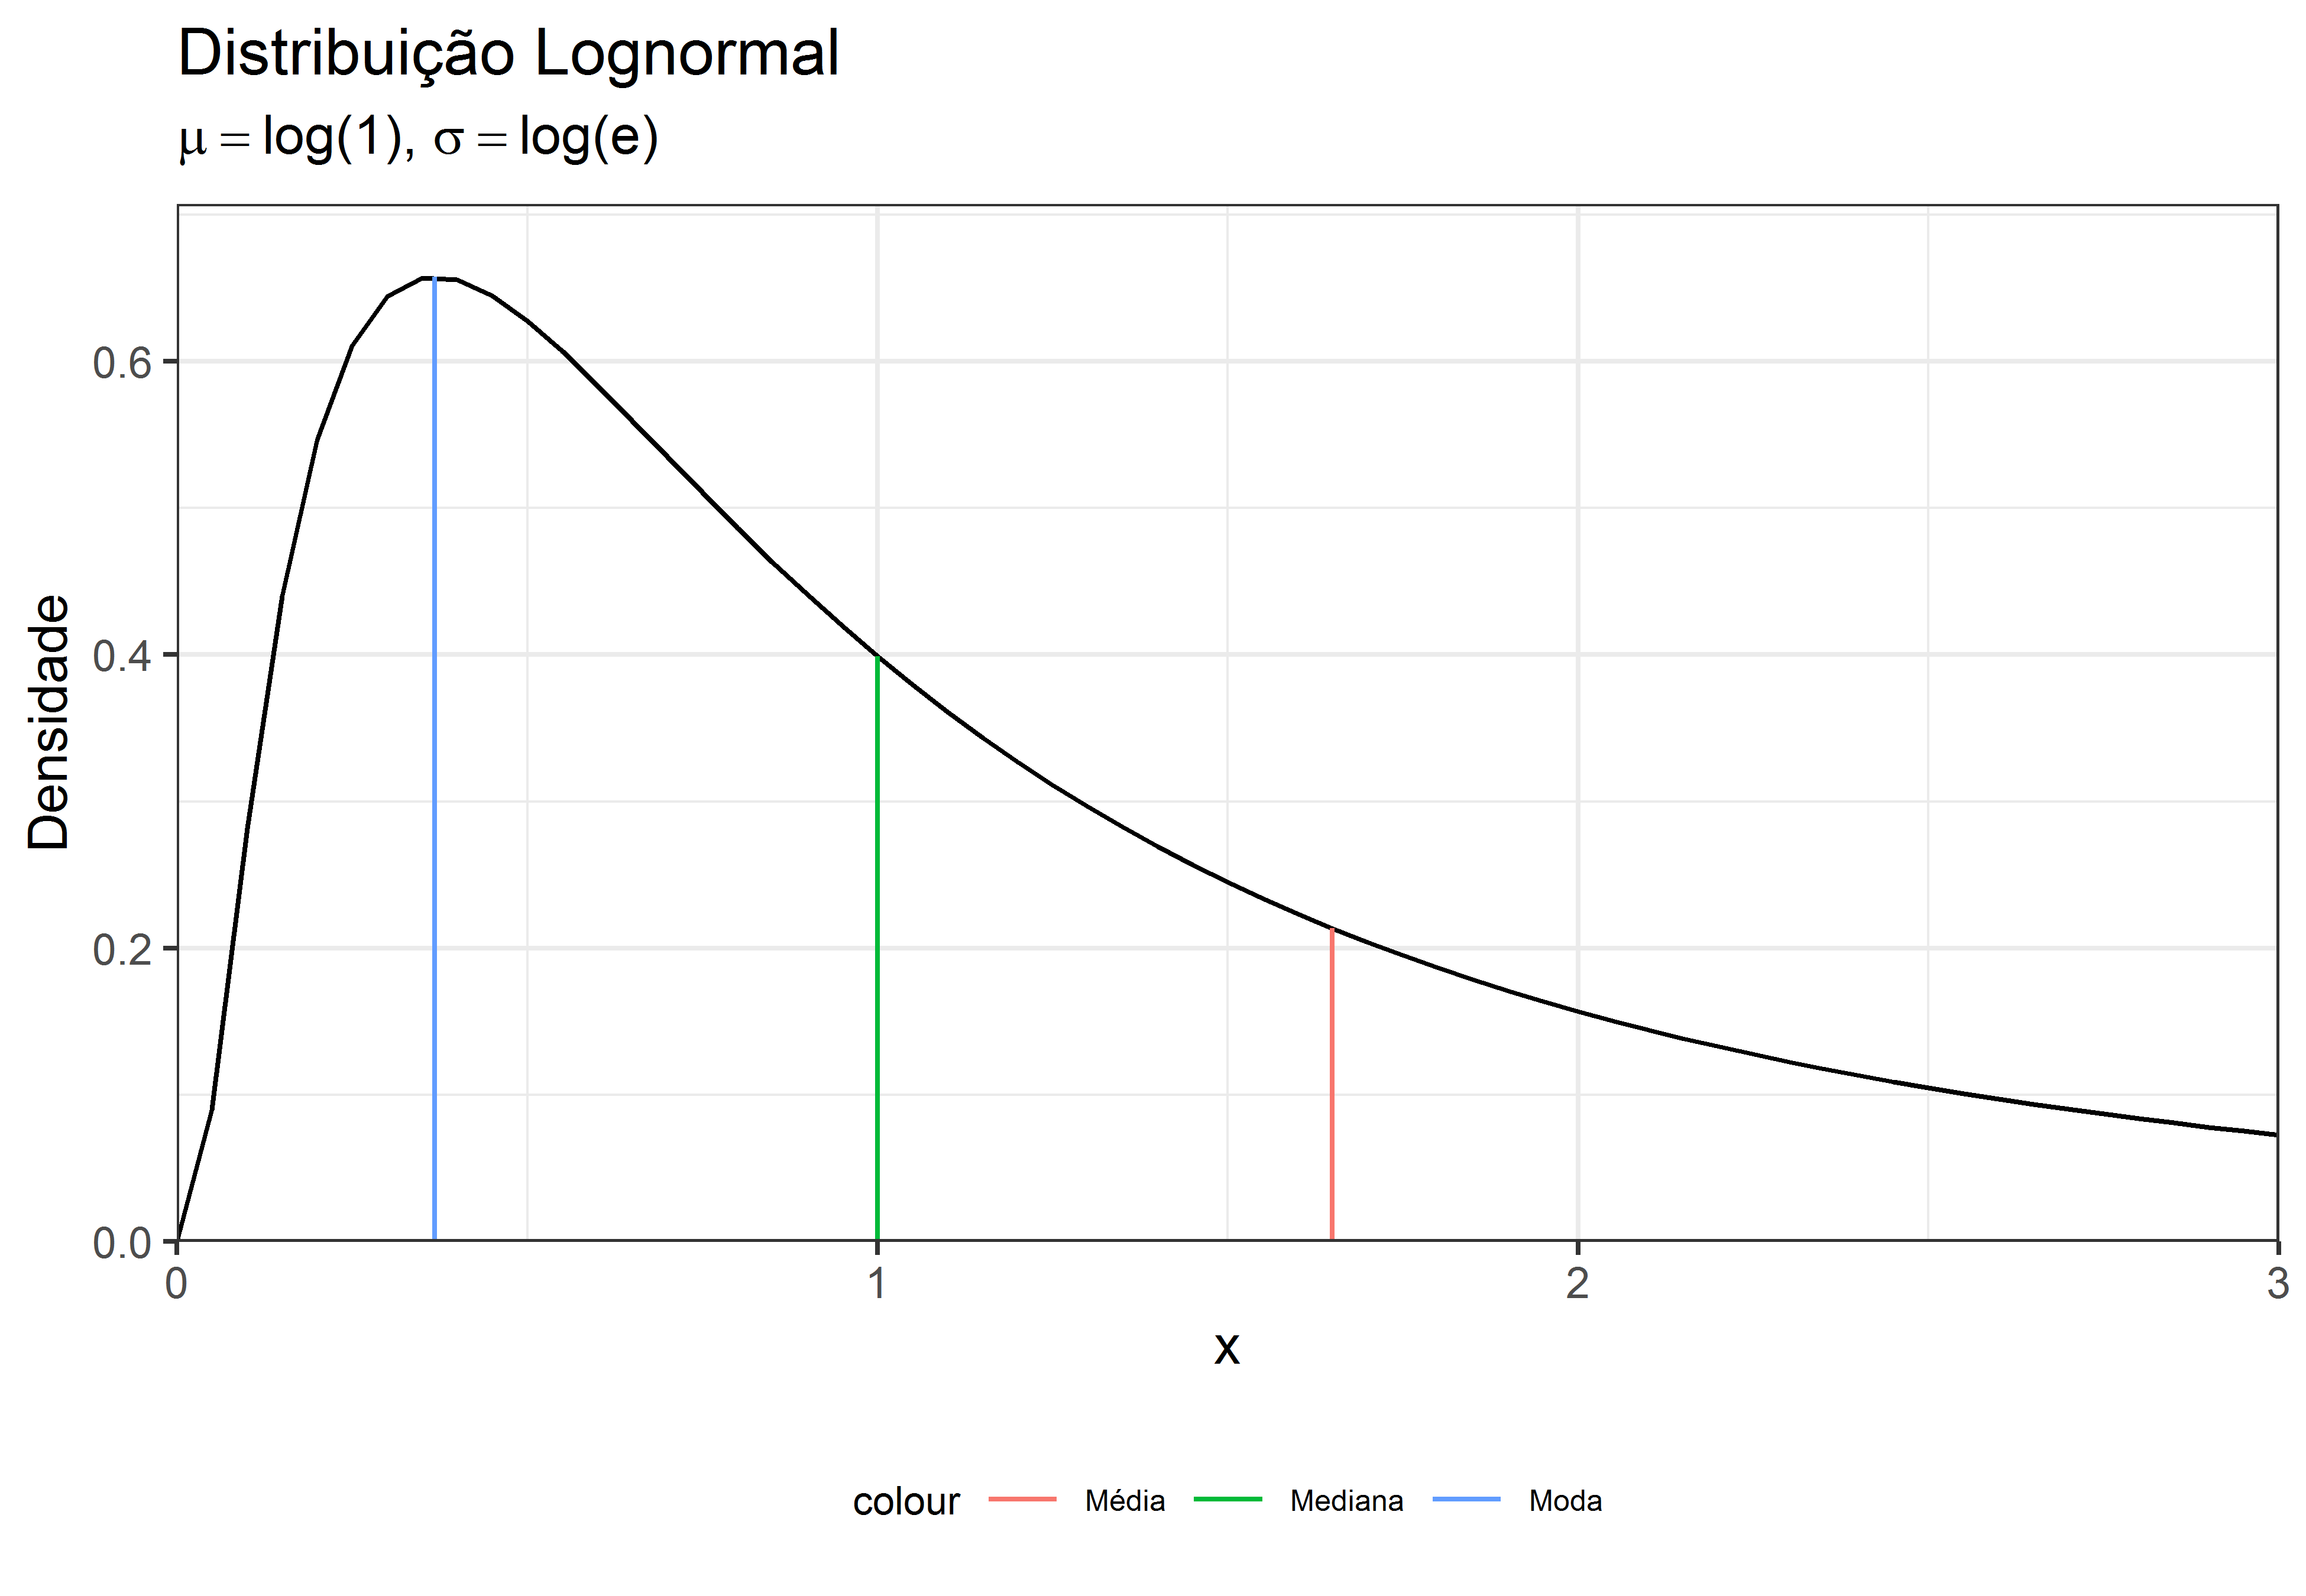
\includegraphics[width=0.7\linewidth]{images/densidade_medidas-1} 

}

\caption{Ilustração das posições de medidas de tendência central numa distribuição lognormal.}\label{fig:densidade_medidas}
\end{figure}

\subsubsection{Efeito das variações do desvio-padrão na forma da
distribuição}\label{efeito-das-variacoes-do-desvio-padrao-na-forma-da-distribuicao}

\begin{figure}[H]

{\centering 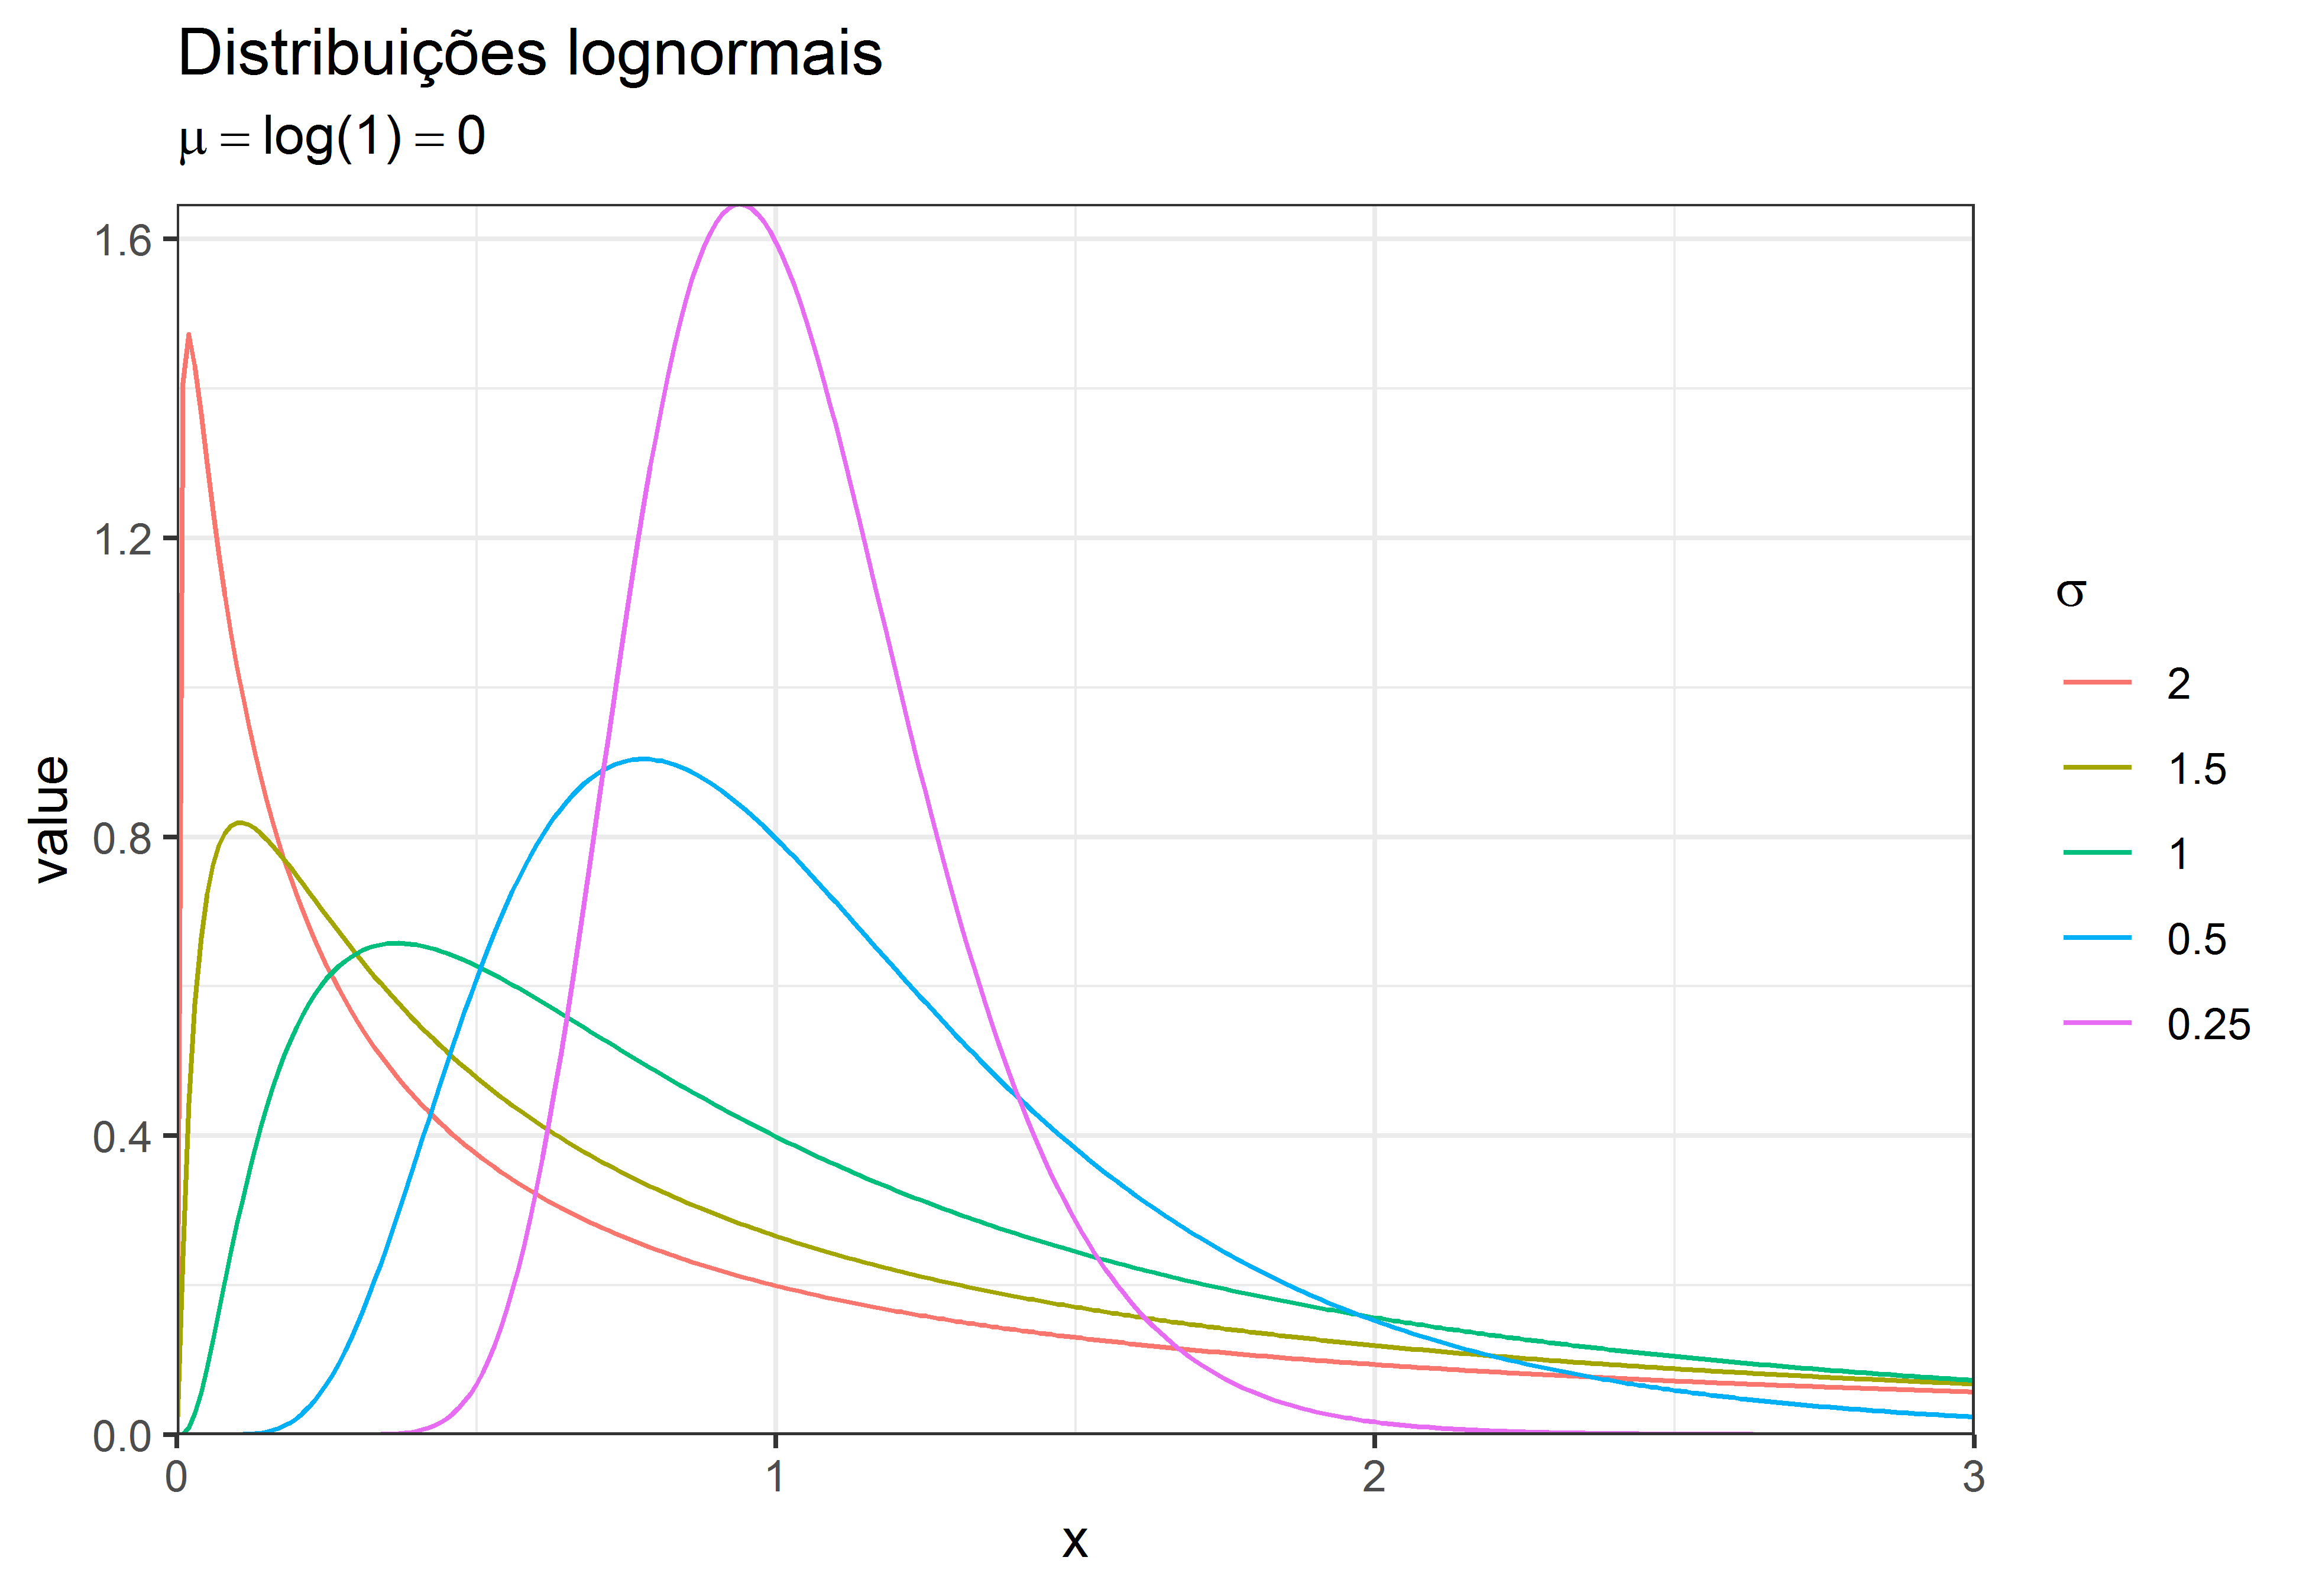
\includegraphics[width=0.7\linewidth]{images/logs-1} 

}

\caption{Distribuição lognormal com $\mu = 0$ e diversos valores de $\sigma$}\label{fig:logs}
\end{figure}

\subsubsection{Relação com a distribuição
normal}\label{relacao-com-a-distribuicao-normal}

Lembrando que a função densidade de probabilidade de uma variável
aleatória com distribuição normal é dada por:

\[f(t) = \frac{1}{\sigma\sqrt{2\pi}}\mathrm{e}^{-\frac{1}{2}\frac{(t-\mu)^2}{\sigma^2}}\]
E que para a distribuição normal-padrão (\(N(0,1)\)) a função densidade
de probabilidade torna-se:

\[\varphi(t) = \frac{1}{\sqrt{2\pi}}\mathrm{e}^{-\frac{1}{2}t^2}\]

Seja \(X\) uma variável aleatória de distribuição normal padronizada
(\(X \sim N(0, 1)\)), \(f_X\) a função densidade de probabilidade e
\(Y = e^X\). Então (\(F_Y\)) é igual a:

\[F_Y(y) = \mathbb{P}(e^X\leq y) = \mathbb{P}(X \leq ln(Y)) = \int_{-\infty}^{ln(y)}f_X(x)dx = \int_{-\infty}^{ln(y)}\frac{1}{\sqrt{2\pi}}e^{-x^2/2}dx\]
o que equivale a:

\[F_Y(y) = \int_{0}^{y}\frac{1}{x}\frac{1}{\sqrt{2\pi}}e^{-ln(x)^2/2}\]

Ou seja, a distribuição de uma variável \(Y = e^X\), em que
\(X \sim N(0,1)\) é equivalente a distribuição de uma variável lognormal
com parâmetros \(\mu = 0\) e \(\sigma = 1\).

A figura \ref{fig:normal_lognormal} ilustra este fato.

\begin{figure}[H]

{\centering 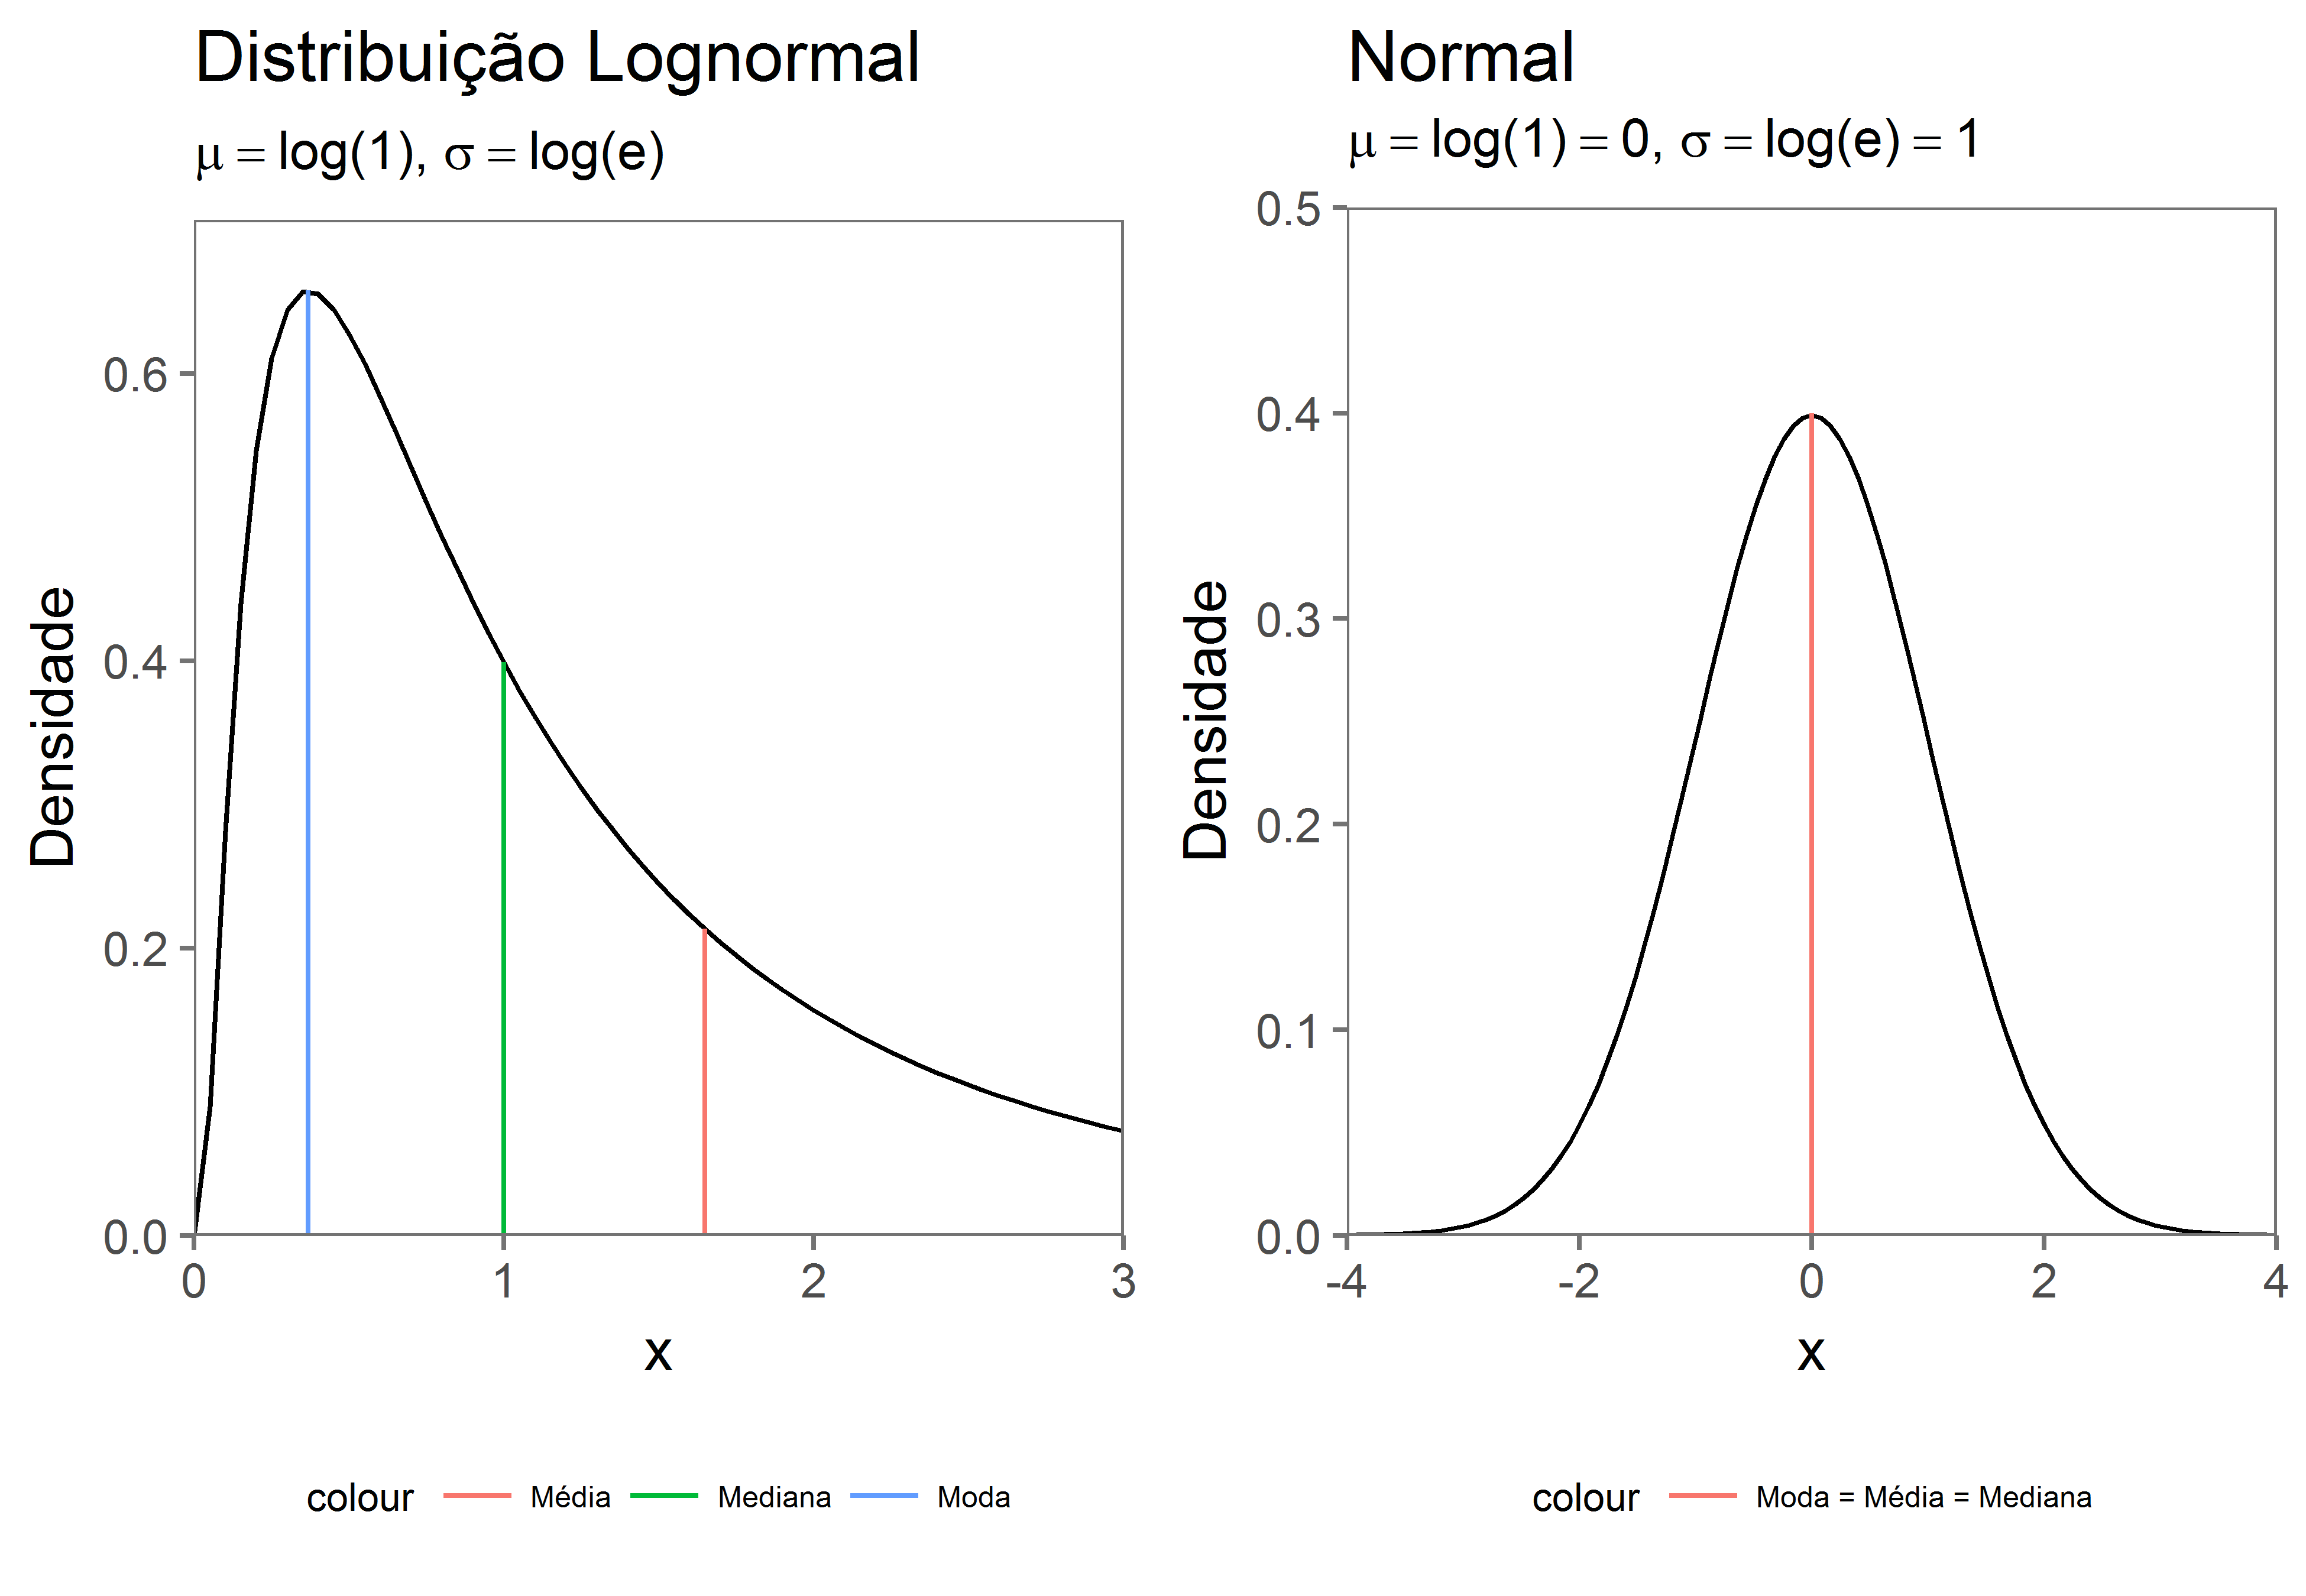
\includegraphics[width=1\linewidth]{images/normal_lognormal-1} 

}

\caption{Comparação entre distribuições normal e lognormal padronizadas.}\label{fig:normal_lognormal}
\end{figure}

\subsubsection{Analogia com o Teorema do Limite
Central}\label{analogia-com-o-teorema-do-limite-central}

Assim como o resultado da soma de diversas variáveis independentes com
distribuições quaisquer resulta numa variável aleatória de distribuição
normal (Teorema do Limite Central), o produto de diversas variáveis
aleatórias resulta numa distribuição lognormal.

\section{EXEMPLO}\label{exemplo}

\subsection{Dados}\label{dados}

Os dados utilizados aqui são oriundos de Hochheim
(\protect\hyperlink{ref-hochheim}{2015}, pp. 21--22) e são reproduzidos
no \protect\hyperlink{anexo-i}{ANEXO I}.

\subsection{Ajuste de distribuições aos
dados}\label{ajuste-de-distribuicoes-aos-dados}

\begin{center}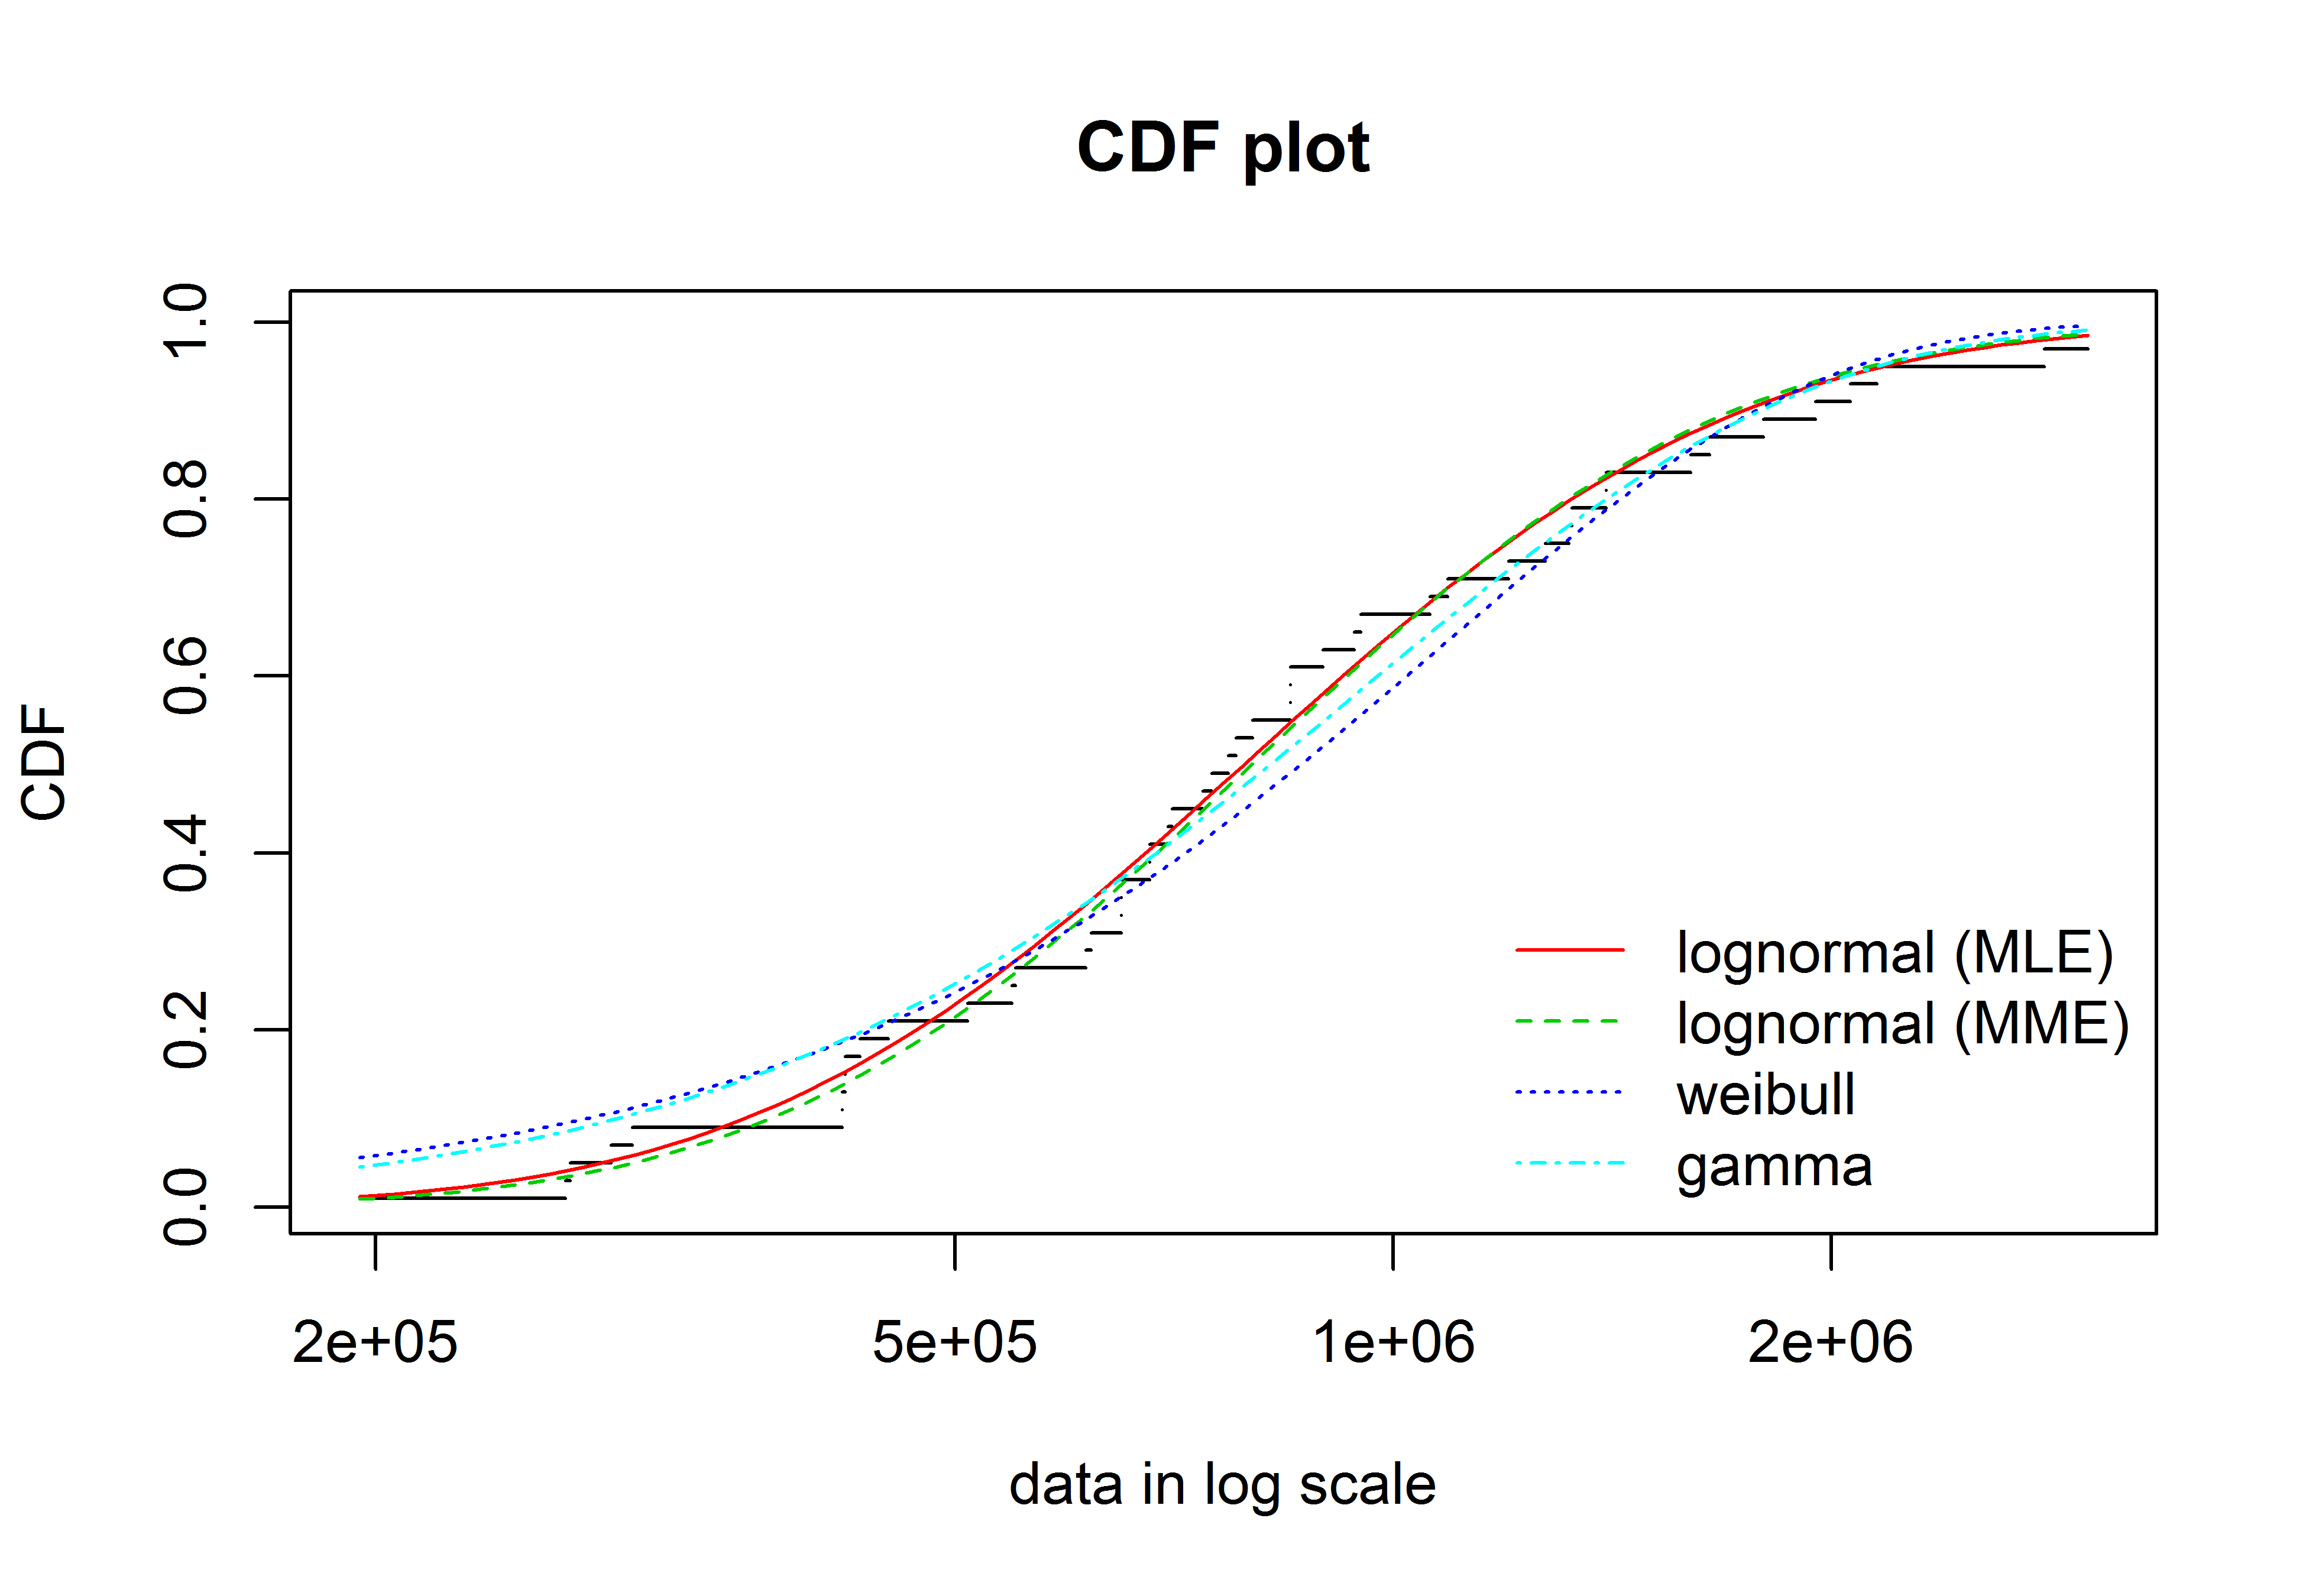
\includegraphics[width=0.49\linewidth]{images/unnamed-chunk-2-1} 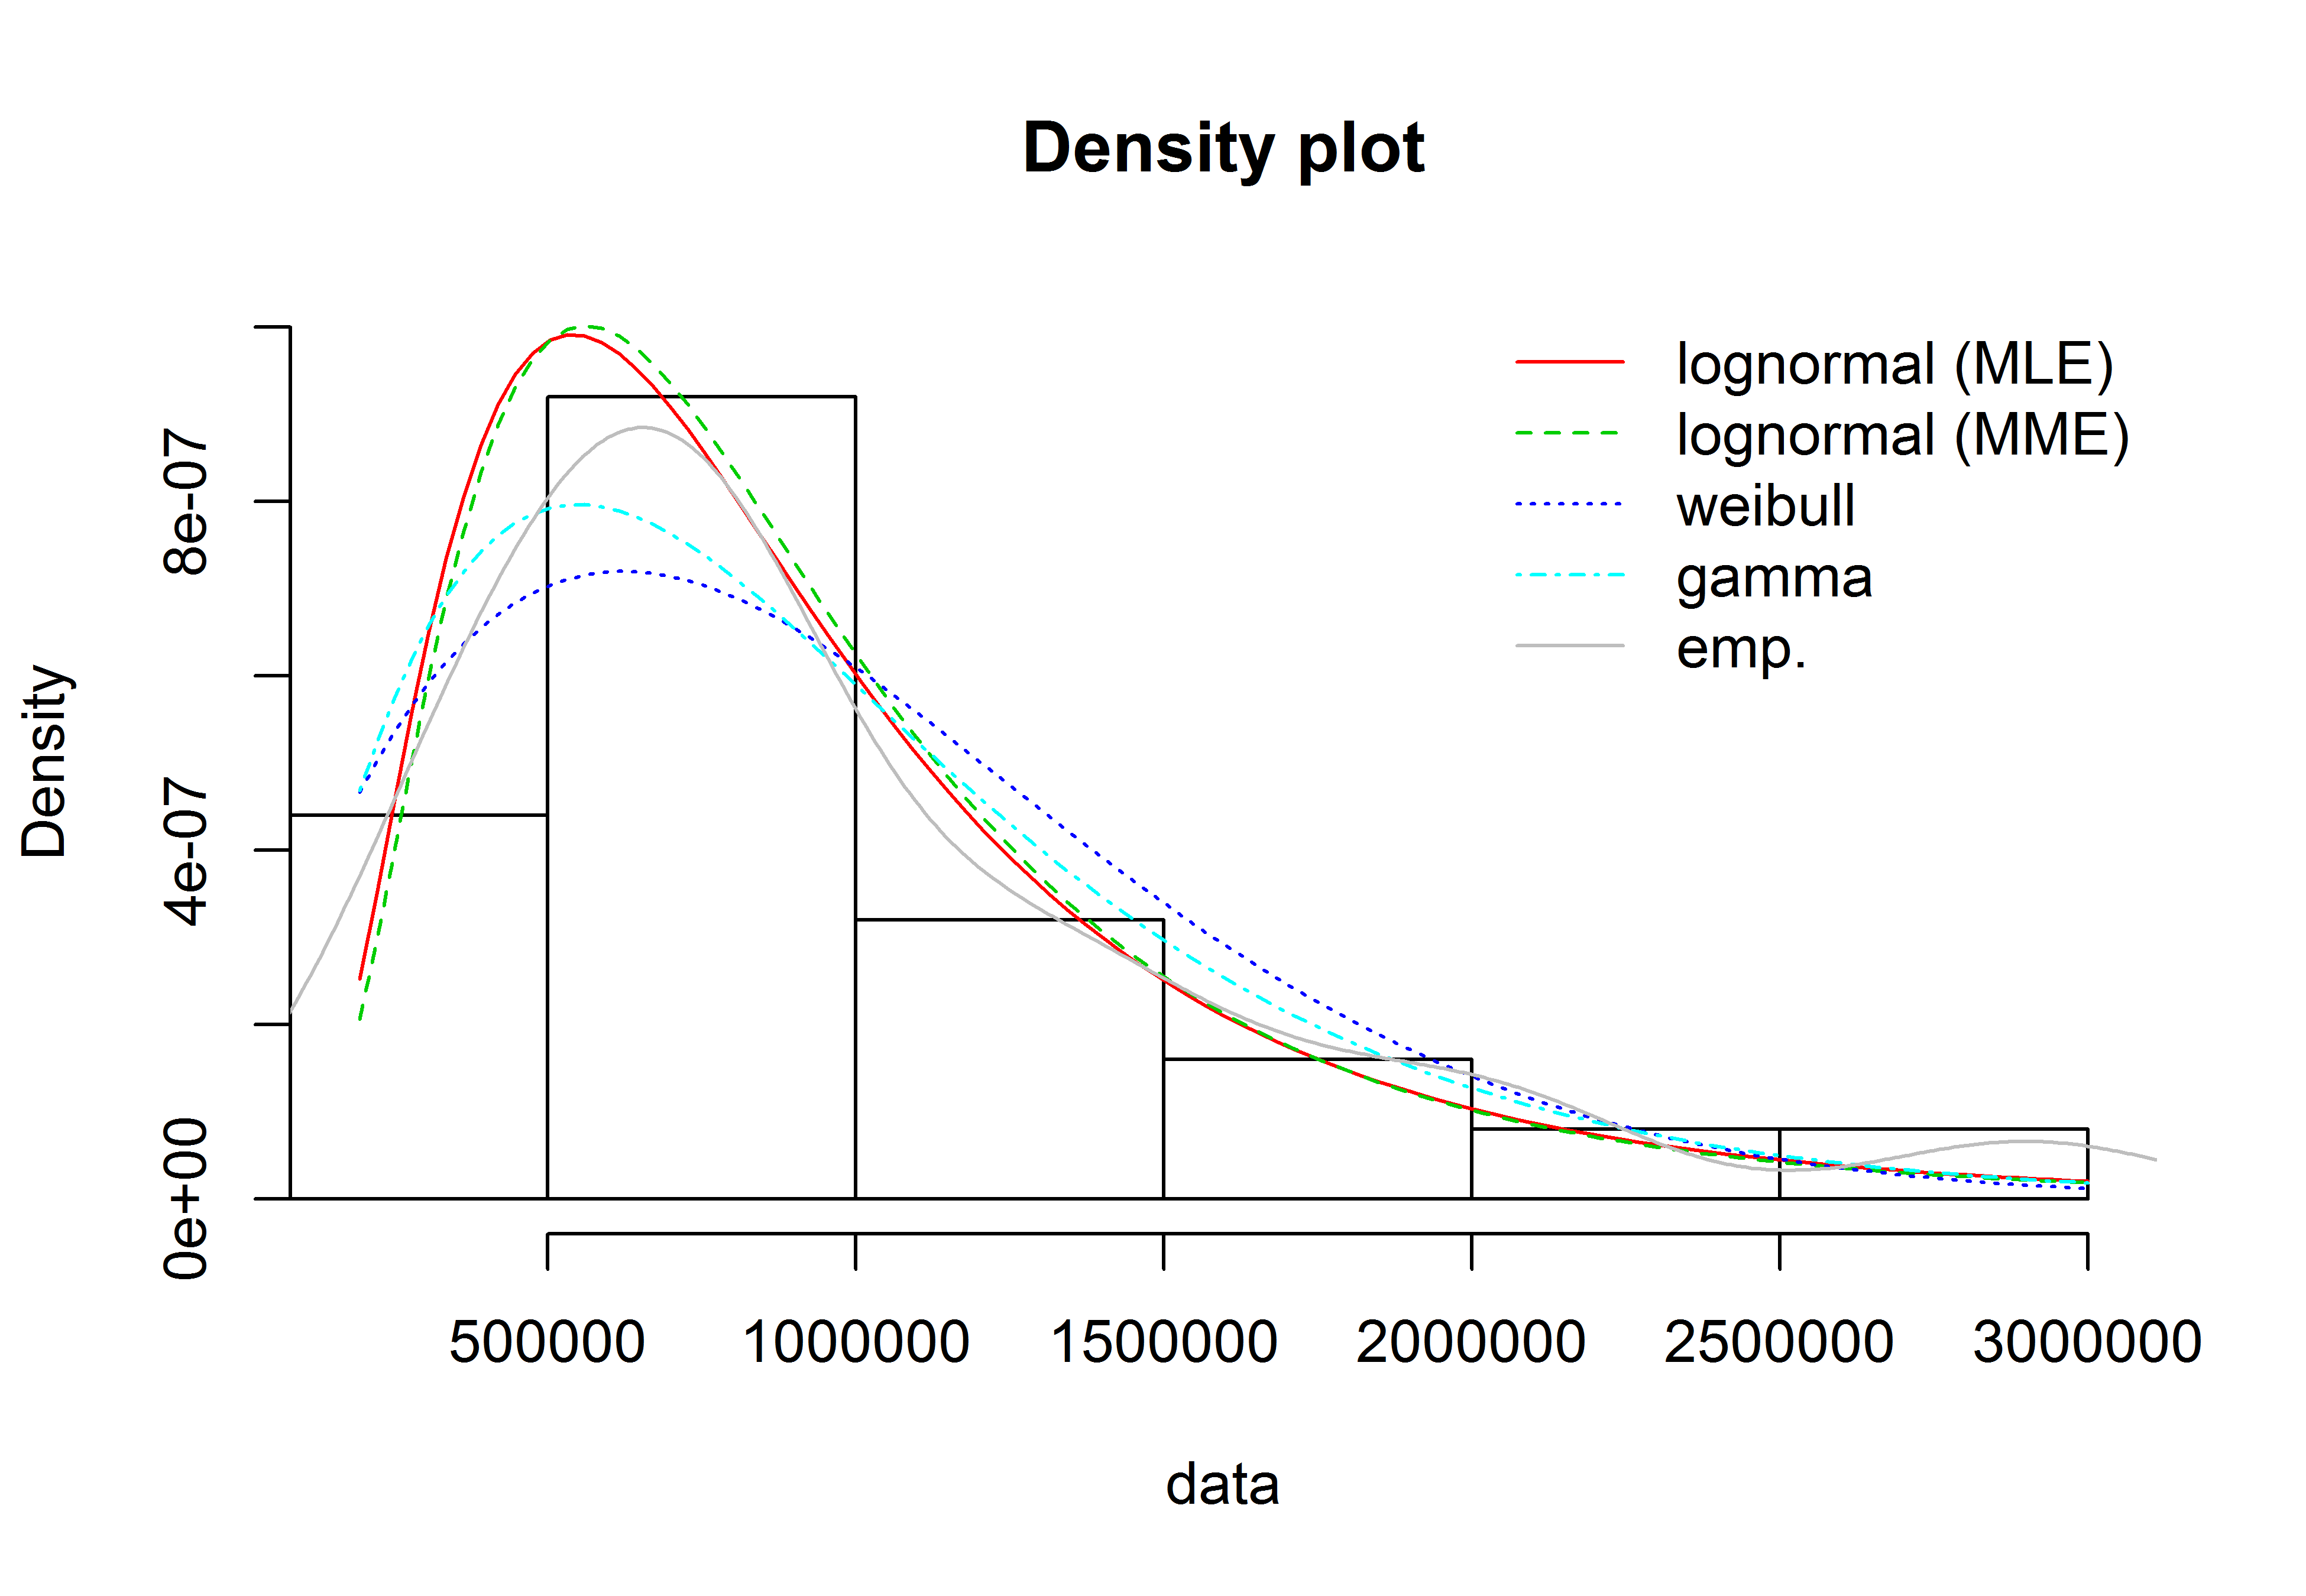
\includegraphics[width=0.49\linewidth]{images/unnamed-chunk-2-2} 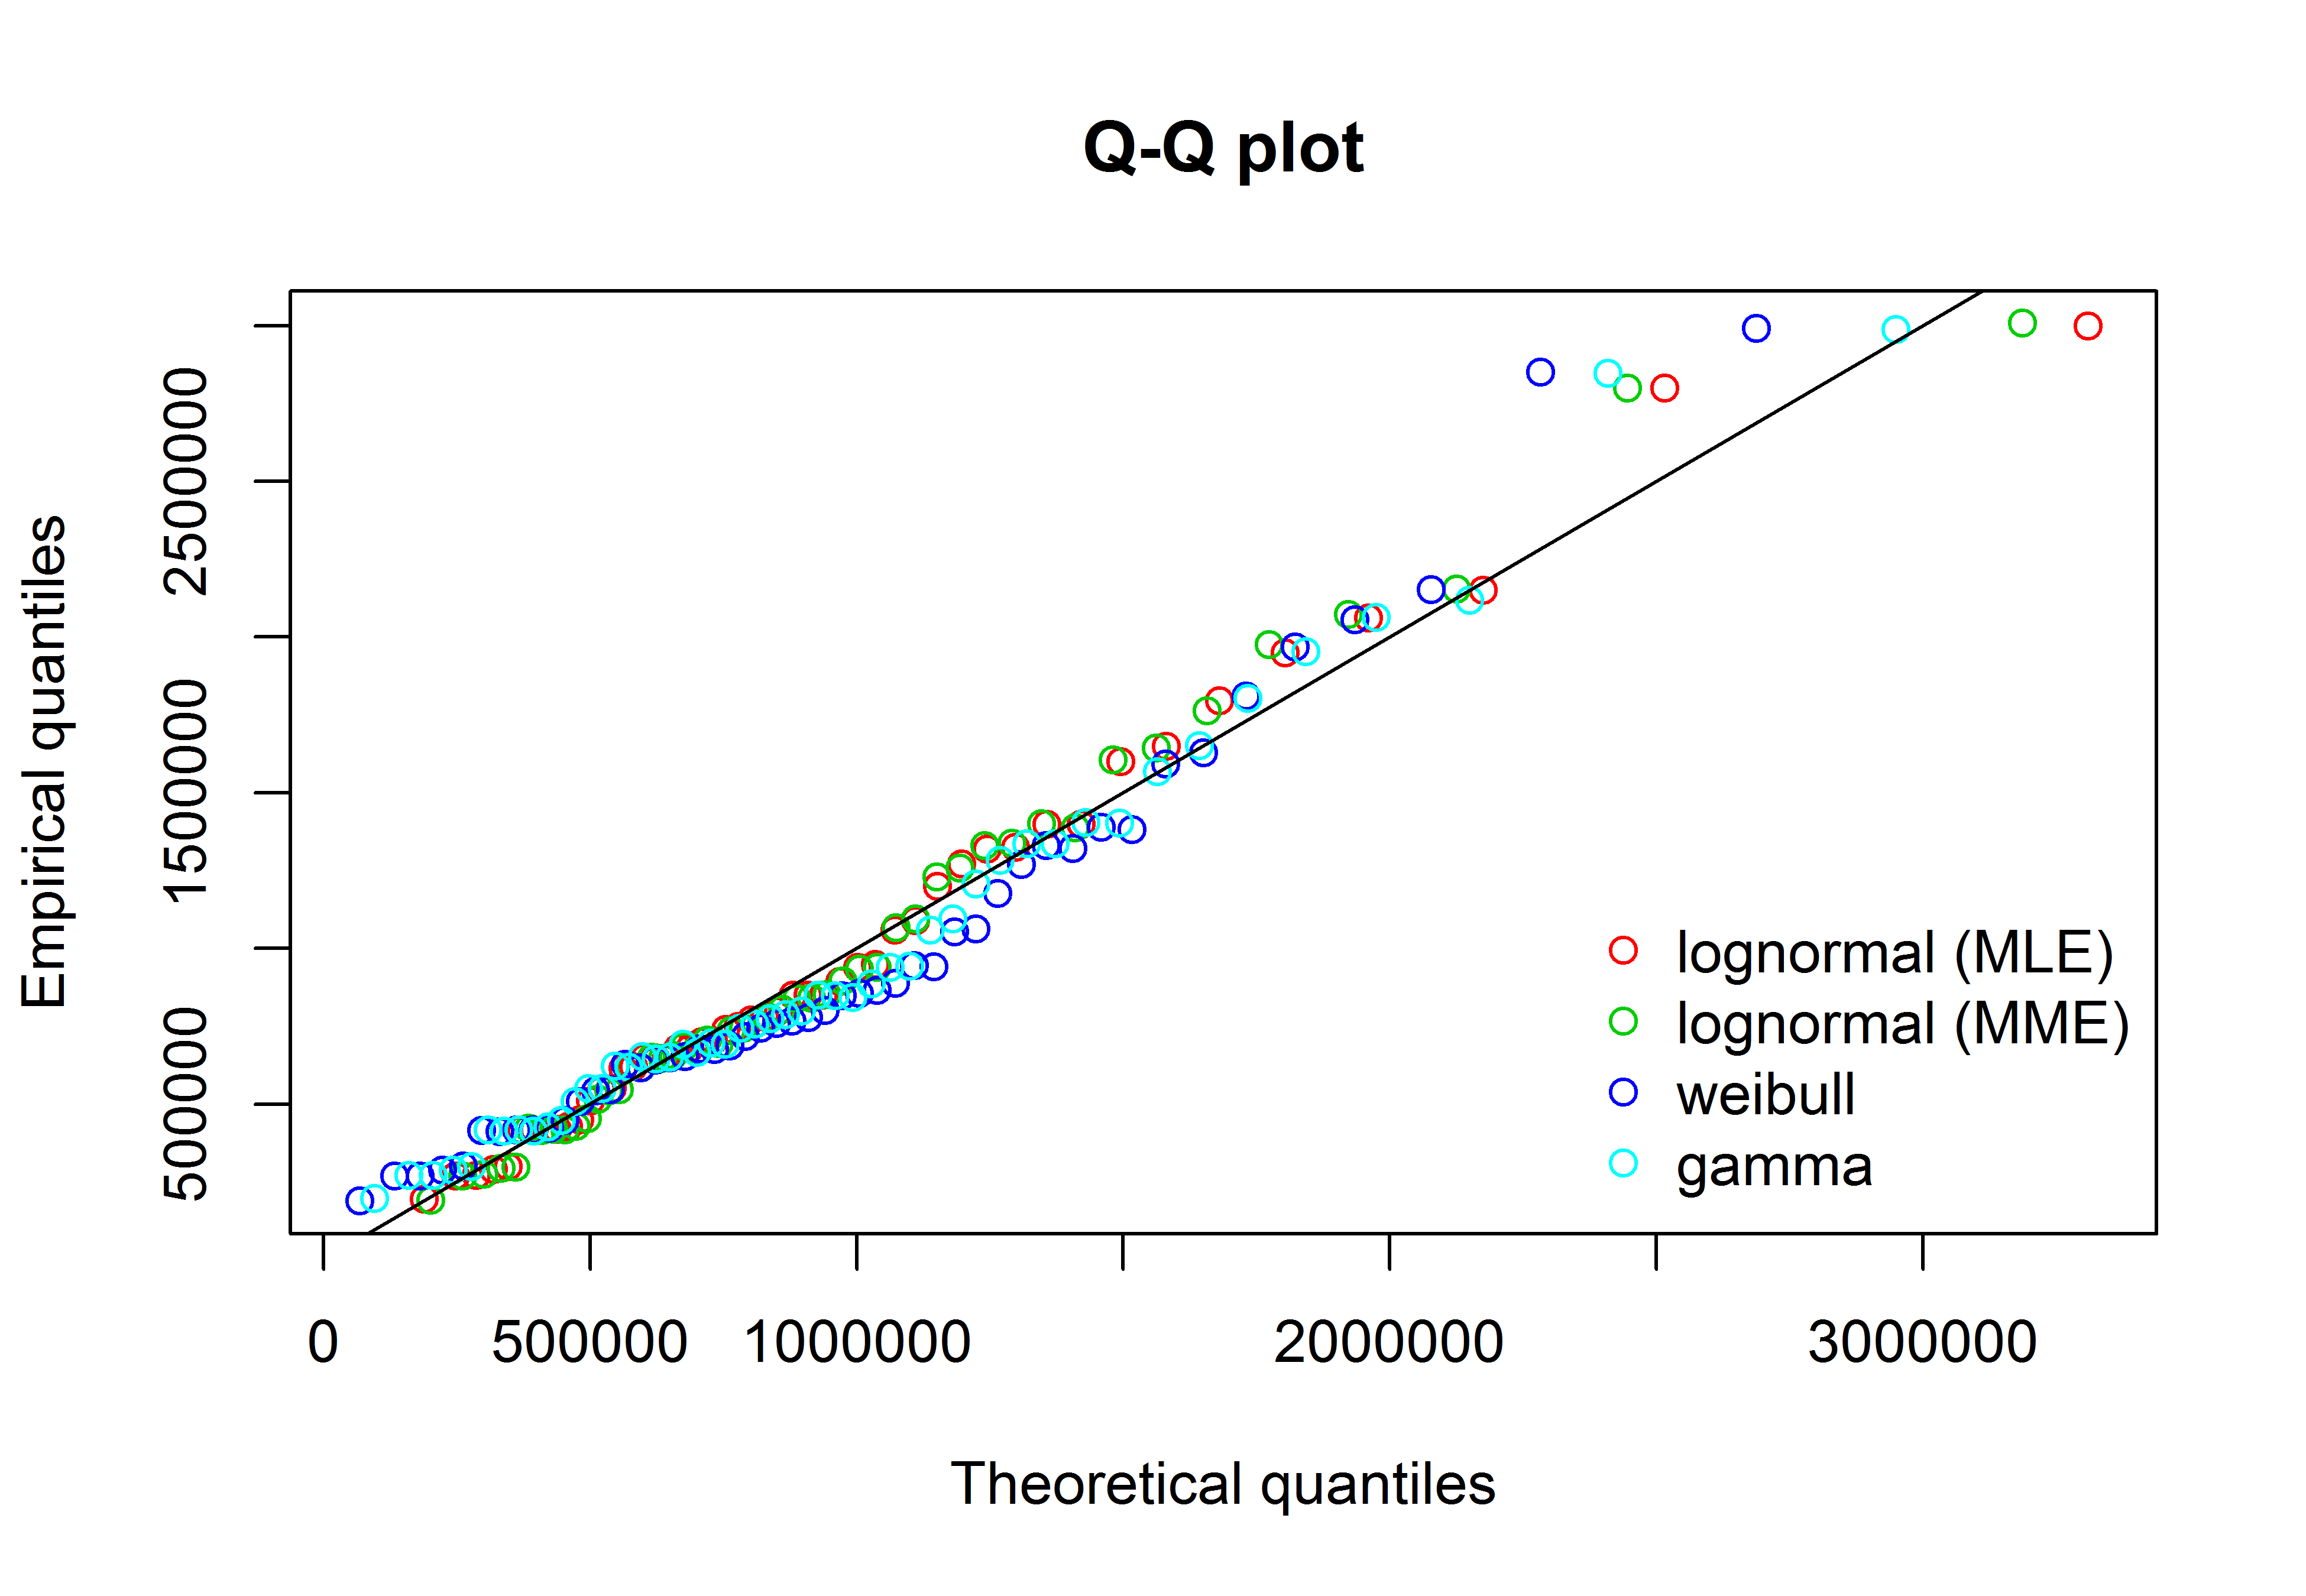
\includegraphics[width=0.49\linewidth]{images/unnamed-chunk-2-3} \end{center}

\subsection{Gráficos}\label{graficos}

As figuras \ref{fig:densidade} e \ref{fig:hist_densidade} mostram que os
valores observados para a variável \code{valor} do conjunto de dados
mencionados acima (HOCHHEIM, \protect\hyperlink{ref-hochheim}{2015}, pp.
21--22) apresentam distribuição aproximadamente lognormal, com
parâmetros \(\mu = \bar{ln(valor)}\)

\newpage

\begin{enumerate}
\def\labelenumi{\alph{enumi}.}
\tightlist
\item
  Densidade
\end{enumerate}

\begin{figure}[H]

{\centering 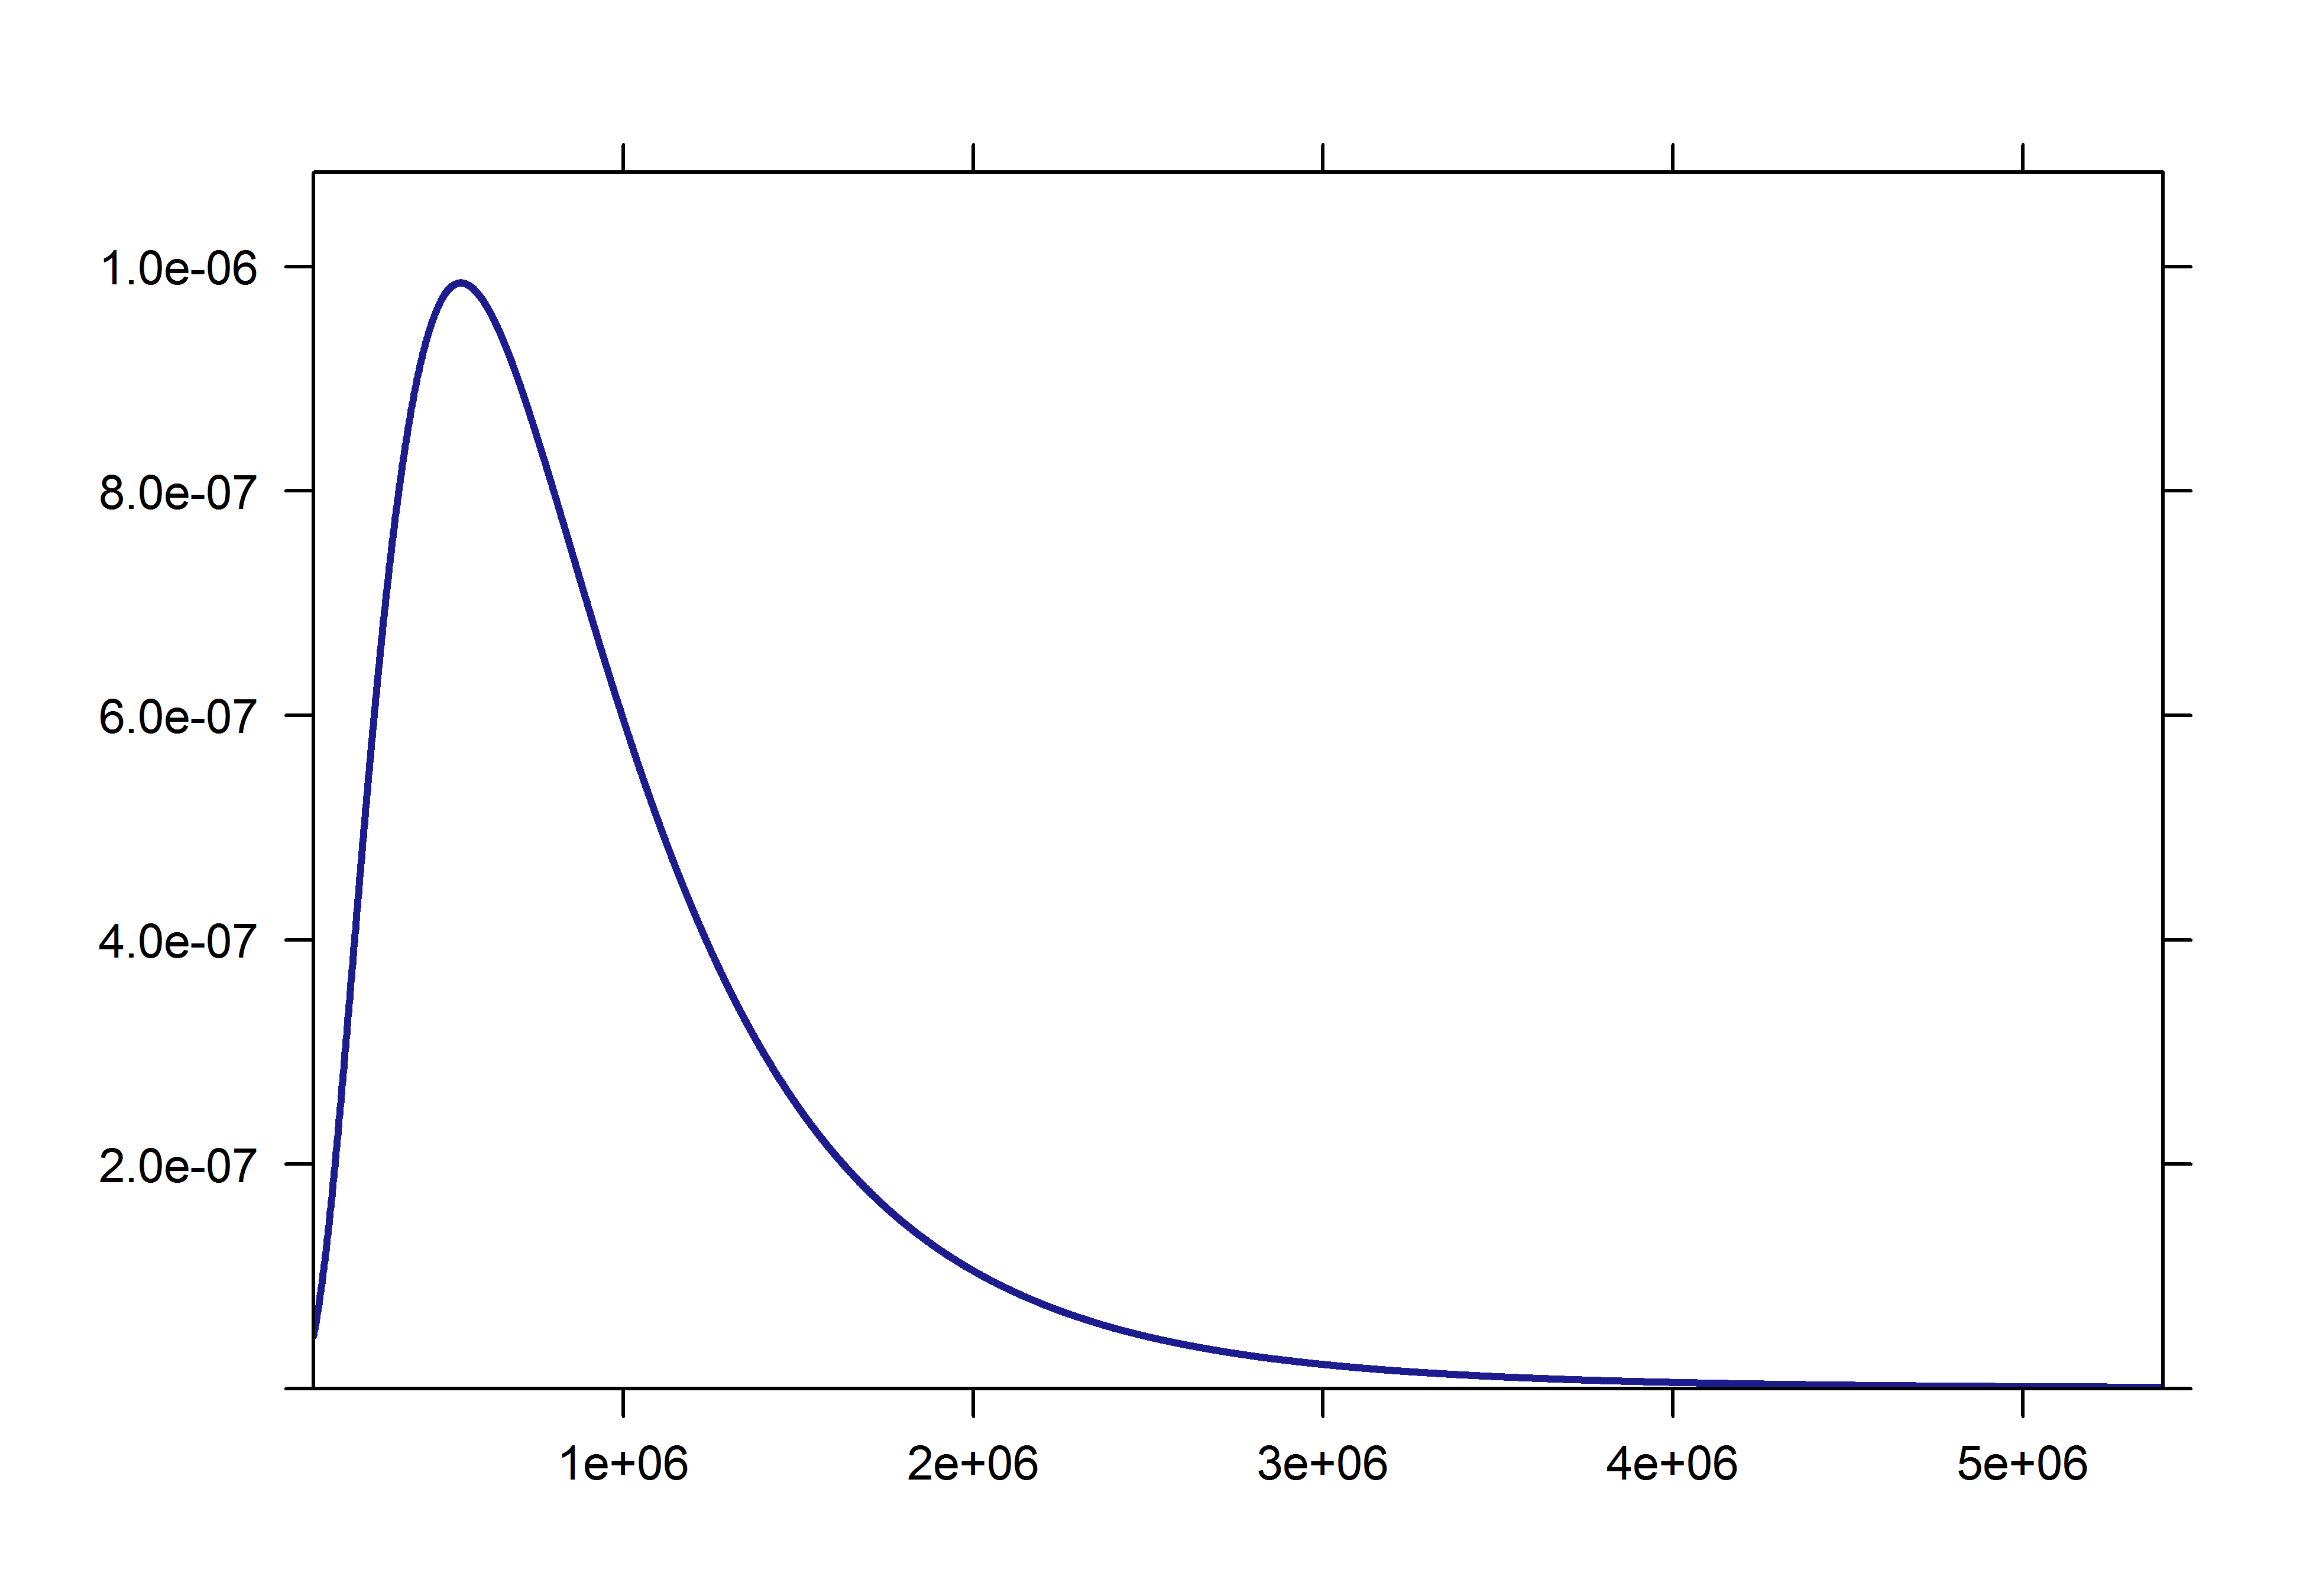
\includegraphics[width=0.7\linewidth]{images/densidade-1} 

}

\caption{Função densidade de probabilidade com parâmetros obtidos dos dados da variável \code{valor}}\label{fig:densidade}
\end{figure}

\begin{enumerate}
\def\labelenumi{\alph{enumi}.}
\setcounter{enumi}{1}
\tightlist
\item
  Histograma com densidade superposta
\end{enumerate}

\begin{figure}[H]

{\centering 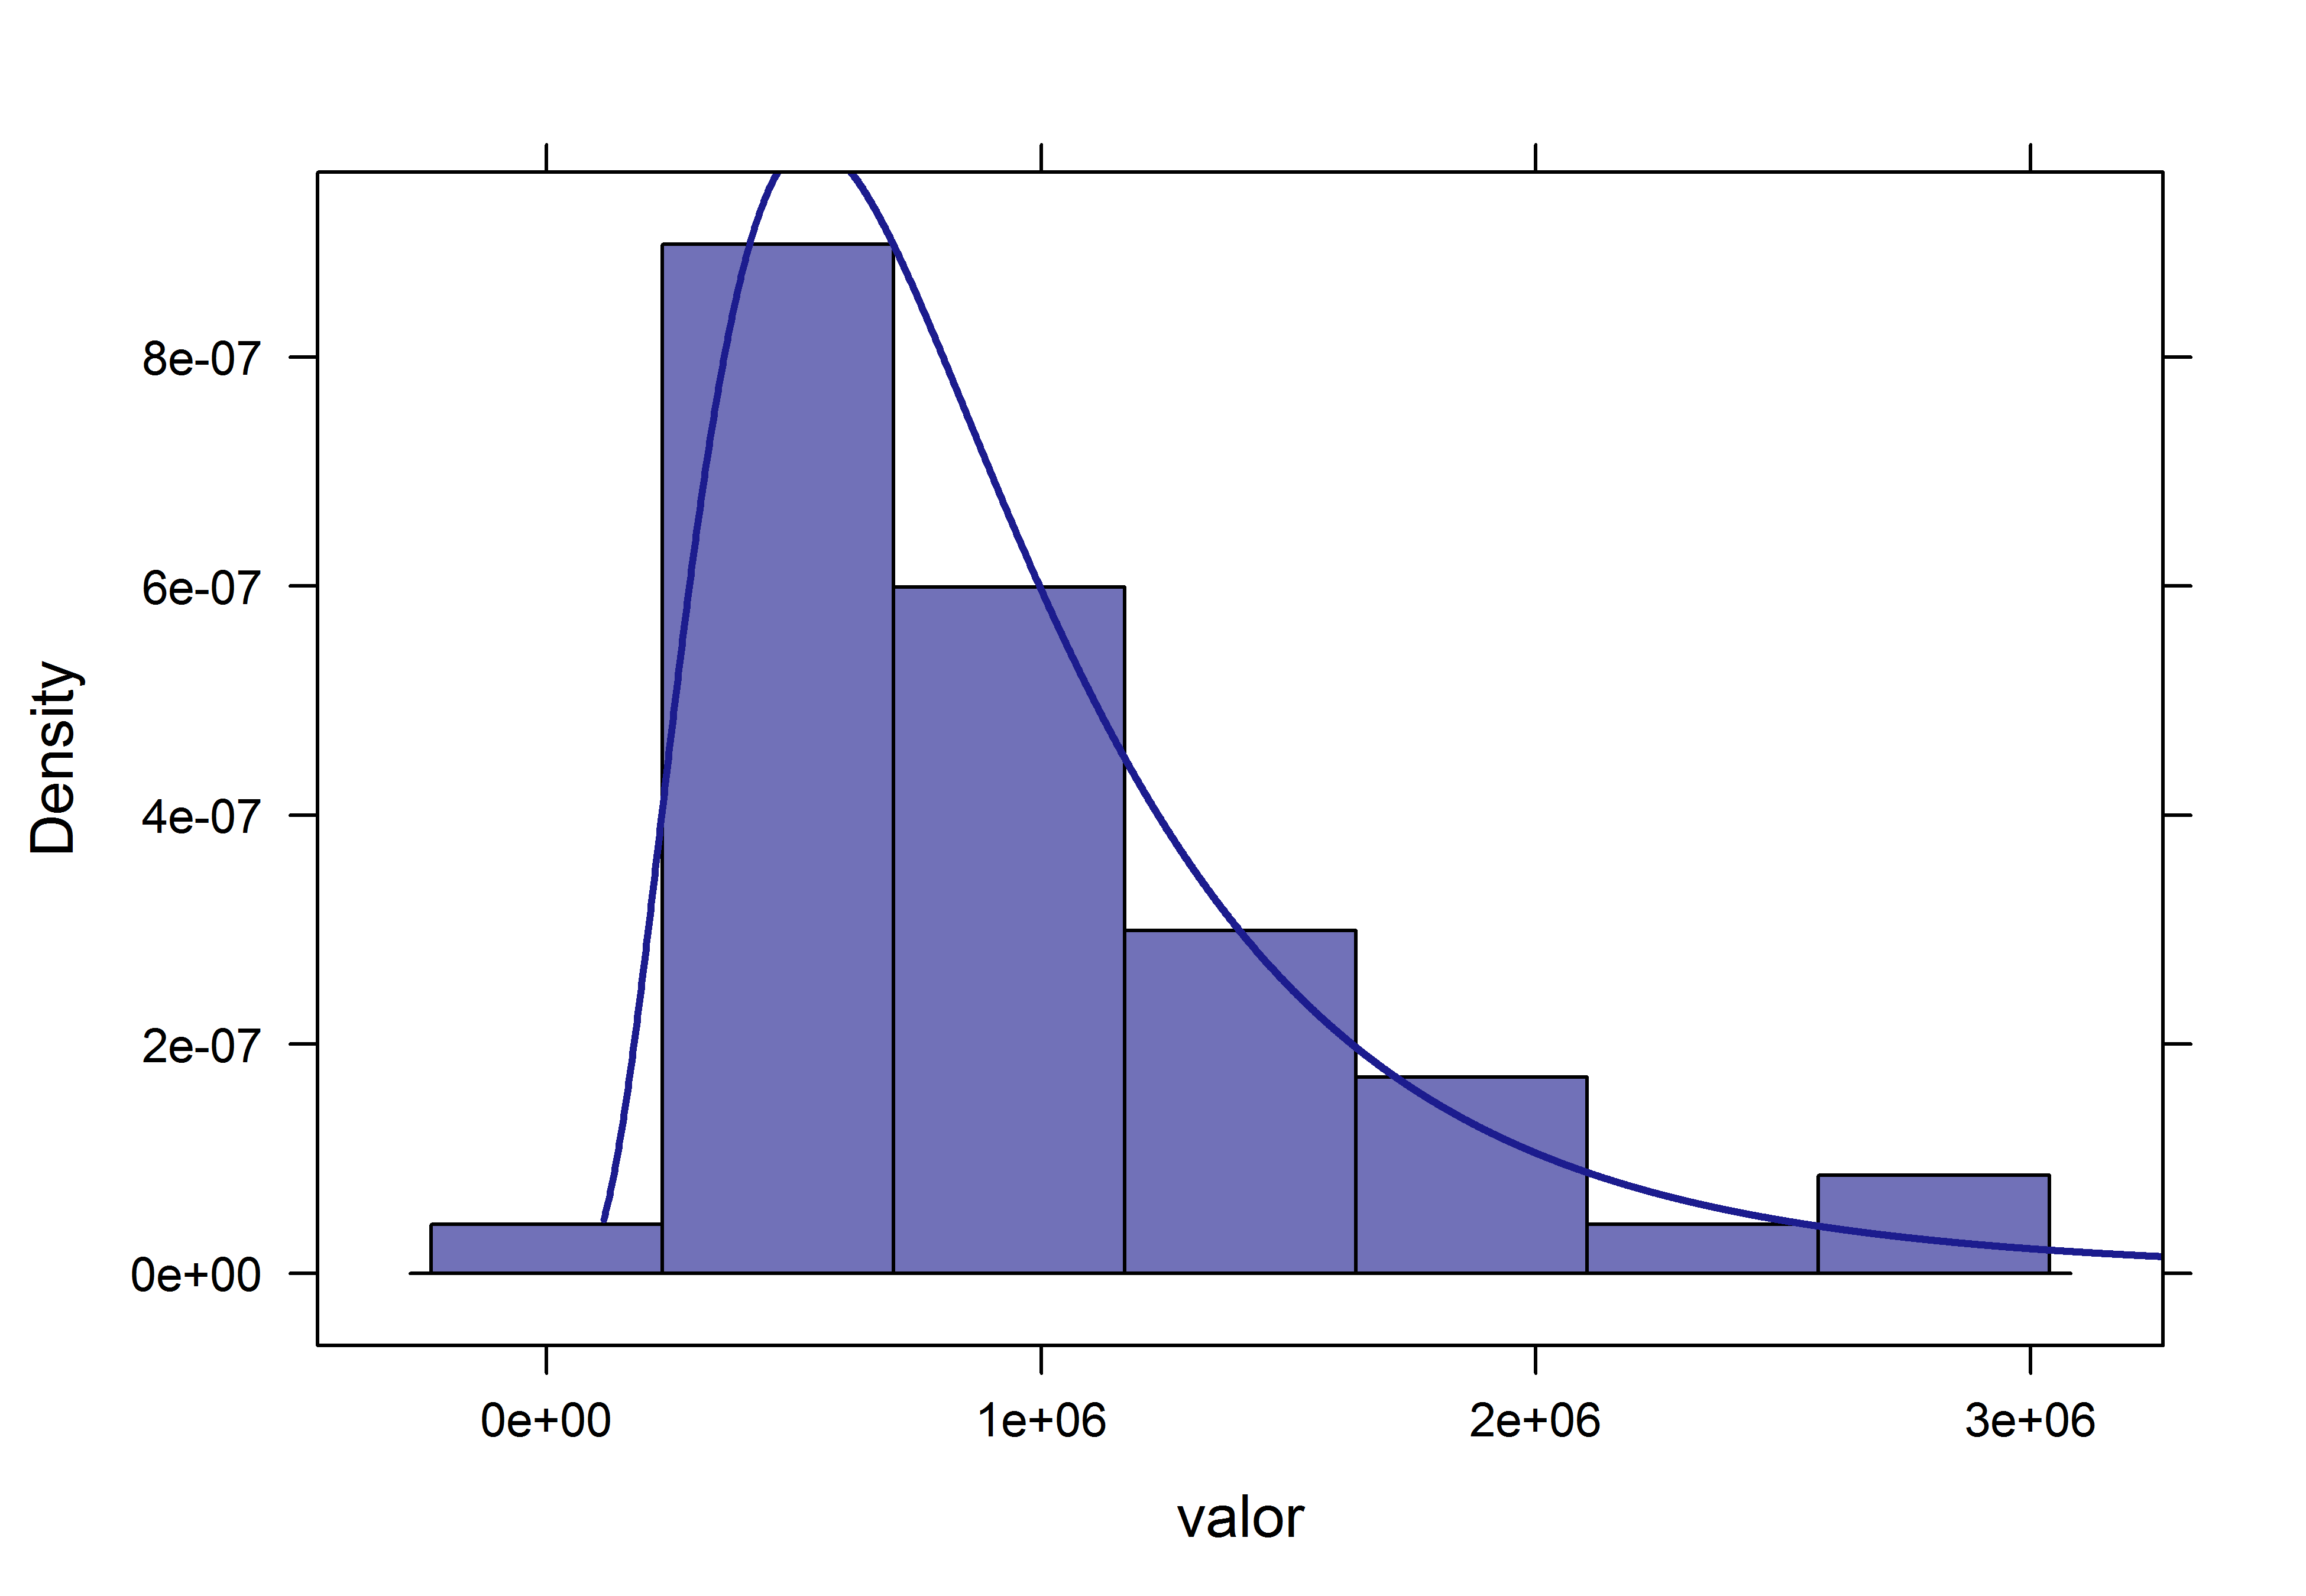
\includegraphics[width=0.7\linewidth]{images/hist_densidade-1} 

}

\caption{Histograma das variável \code{valor} com função densidade de probabilidade superposta.}\label{fig:hist_densidade}
\end{figure}

\begin{enumerate}
\def\labelenumi{\alph{enumi}.}
\setcounter{enumi}{2}
\tightlist
\item
  Cumulativa
\end{enumerate}

\begin{figure}[H]

{\centering 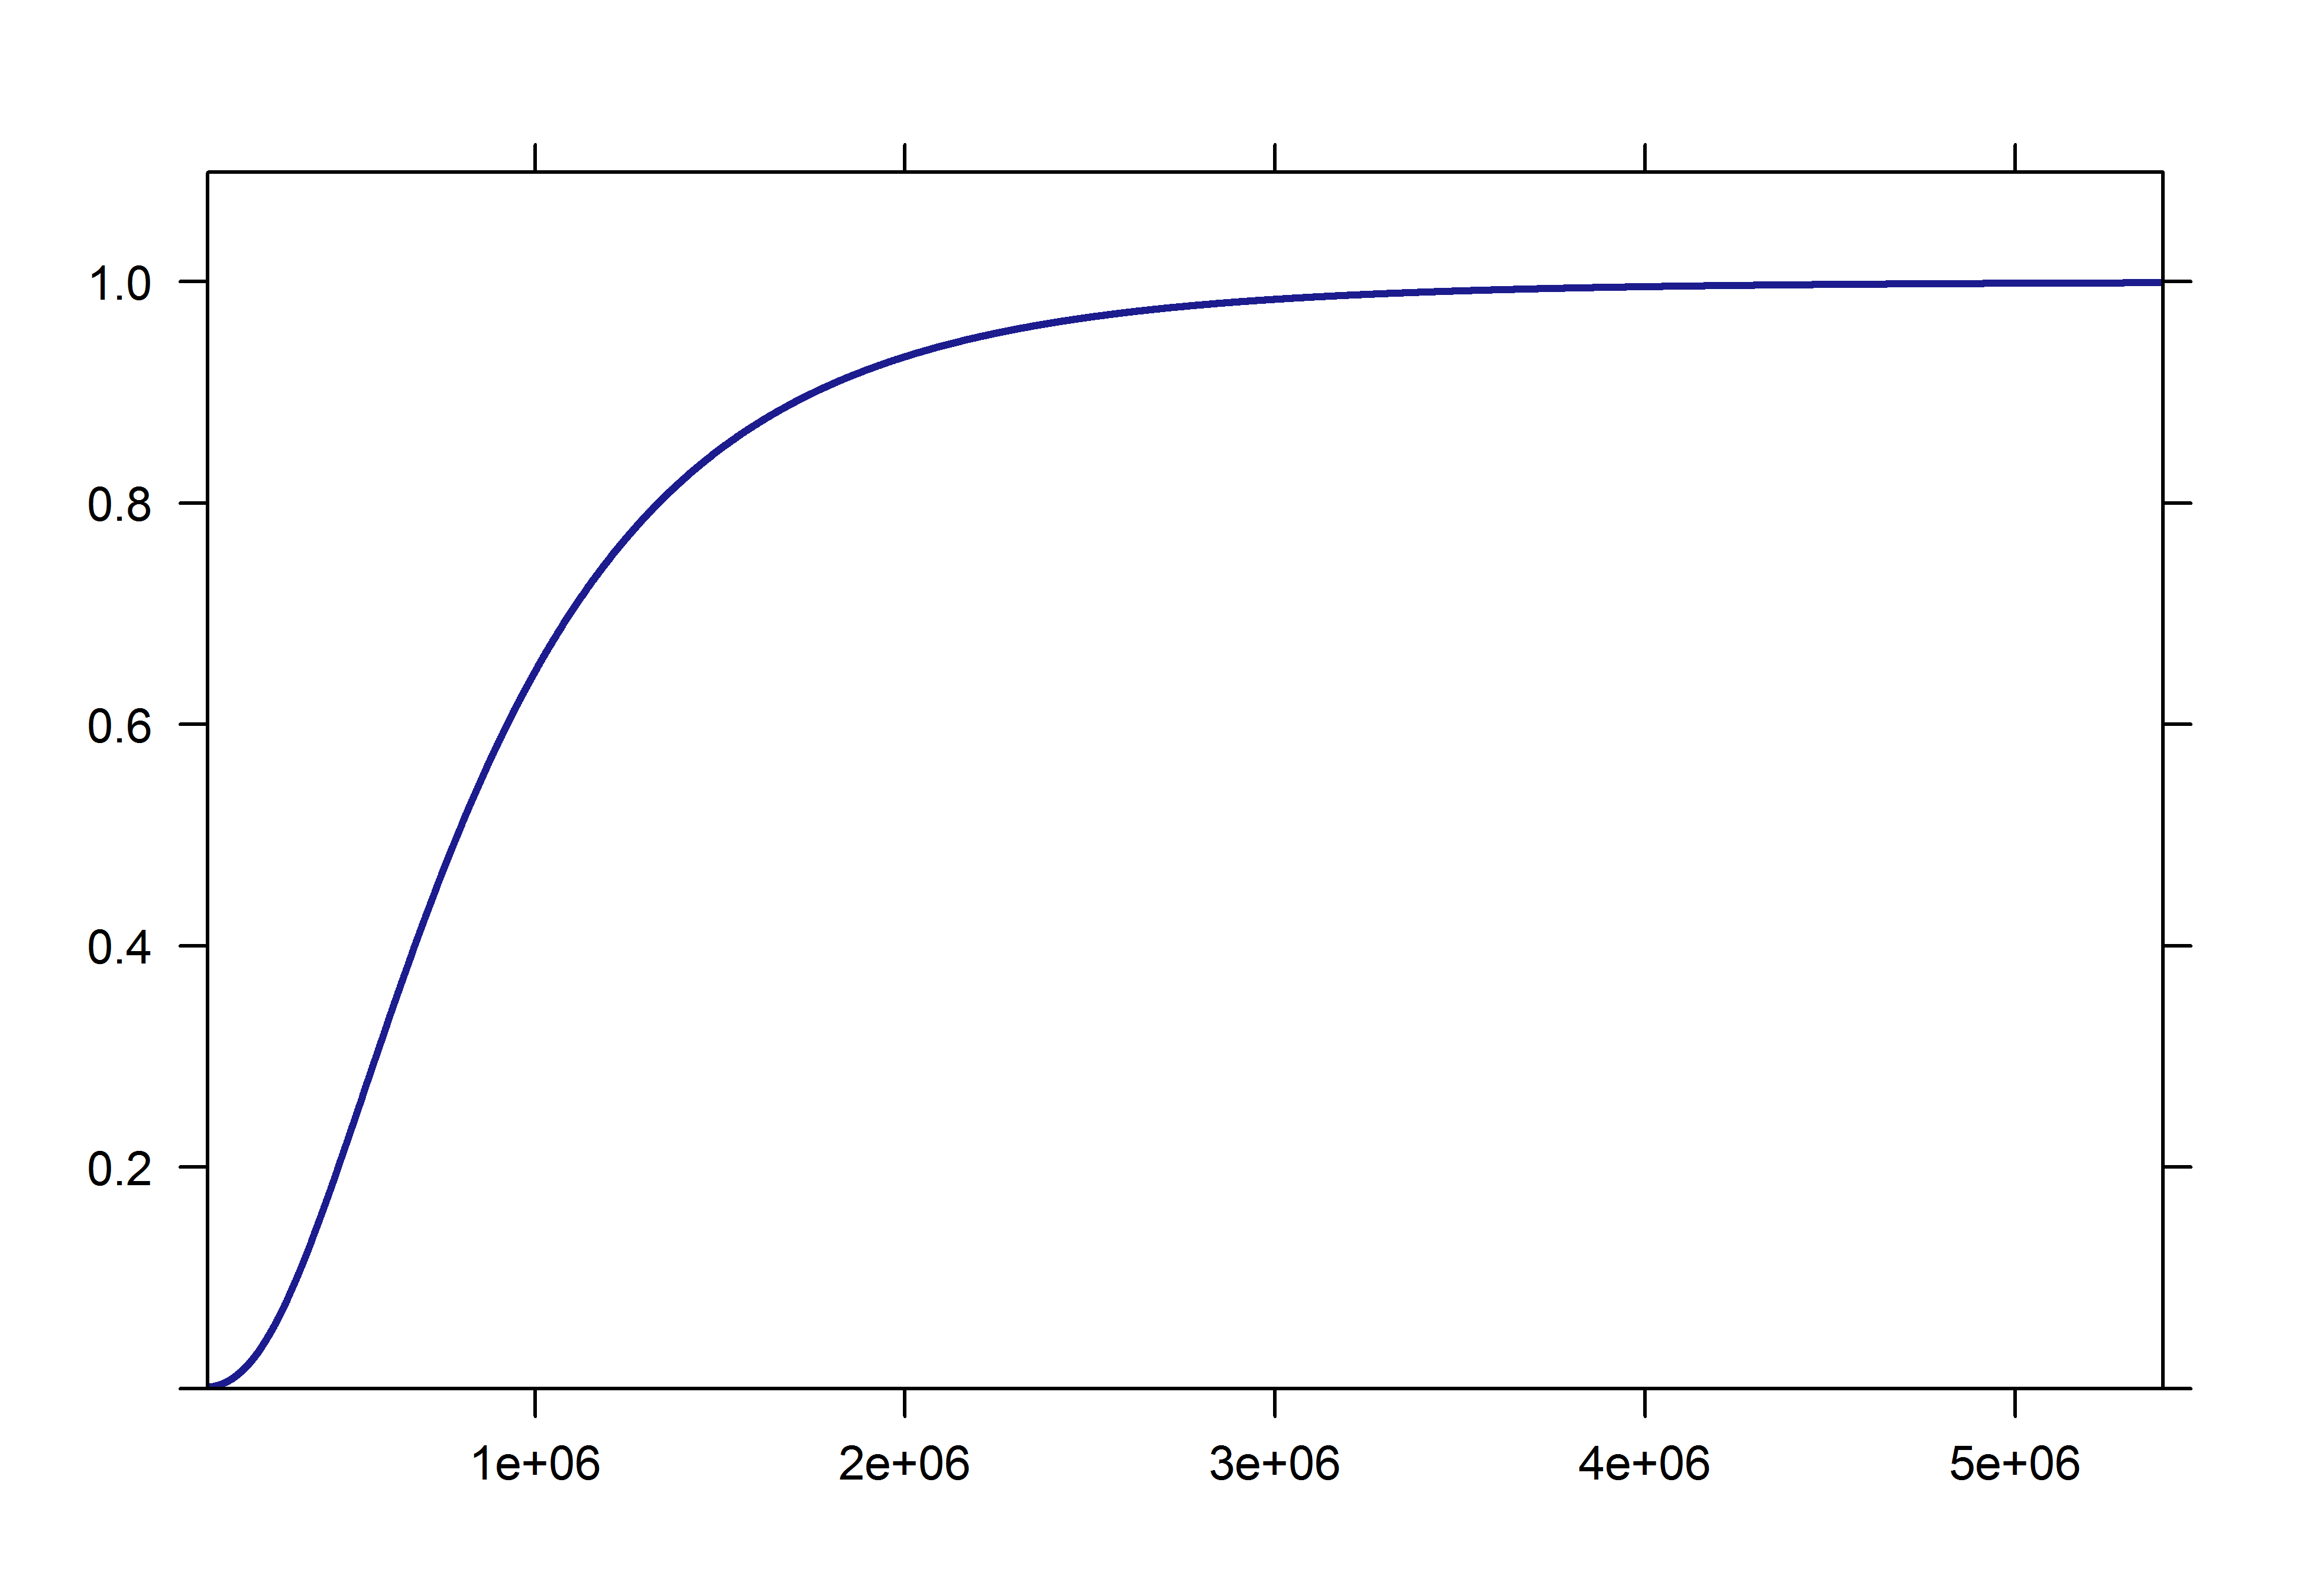
\includegraphics[width=0.7\linewidth]{images/cdf-1} 

}

\caption{Função cumulativa de densidade de probabilidade com parâmetros obtidos dos dados da variável \code{valor}}\label{fig:cdf}
\end{figure}

\begin{enumerate}
\def\labelenumi{\alph{enumi}.}
\setcounter{enumi}{3}
\tightlist
\item
  Distribuição da variável \(ln(valor)\)
\end{enumerate}

A figura \ref{fig:hist_densidade2}

\begin{figure}[H]

{\centering 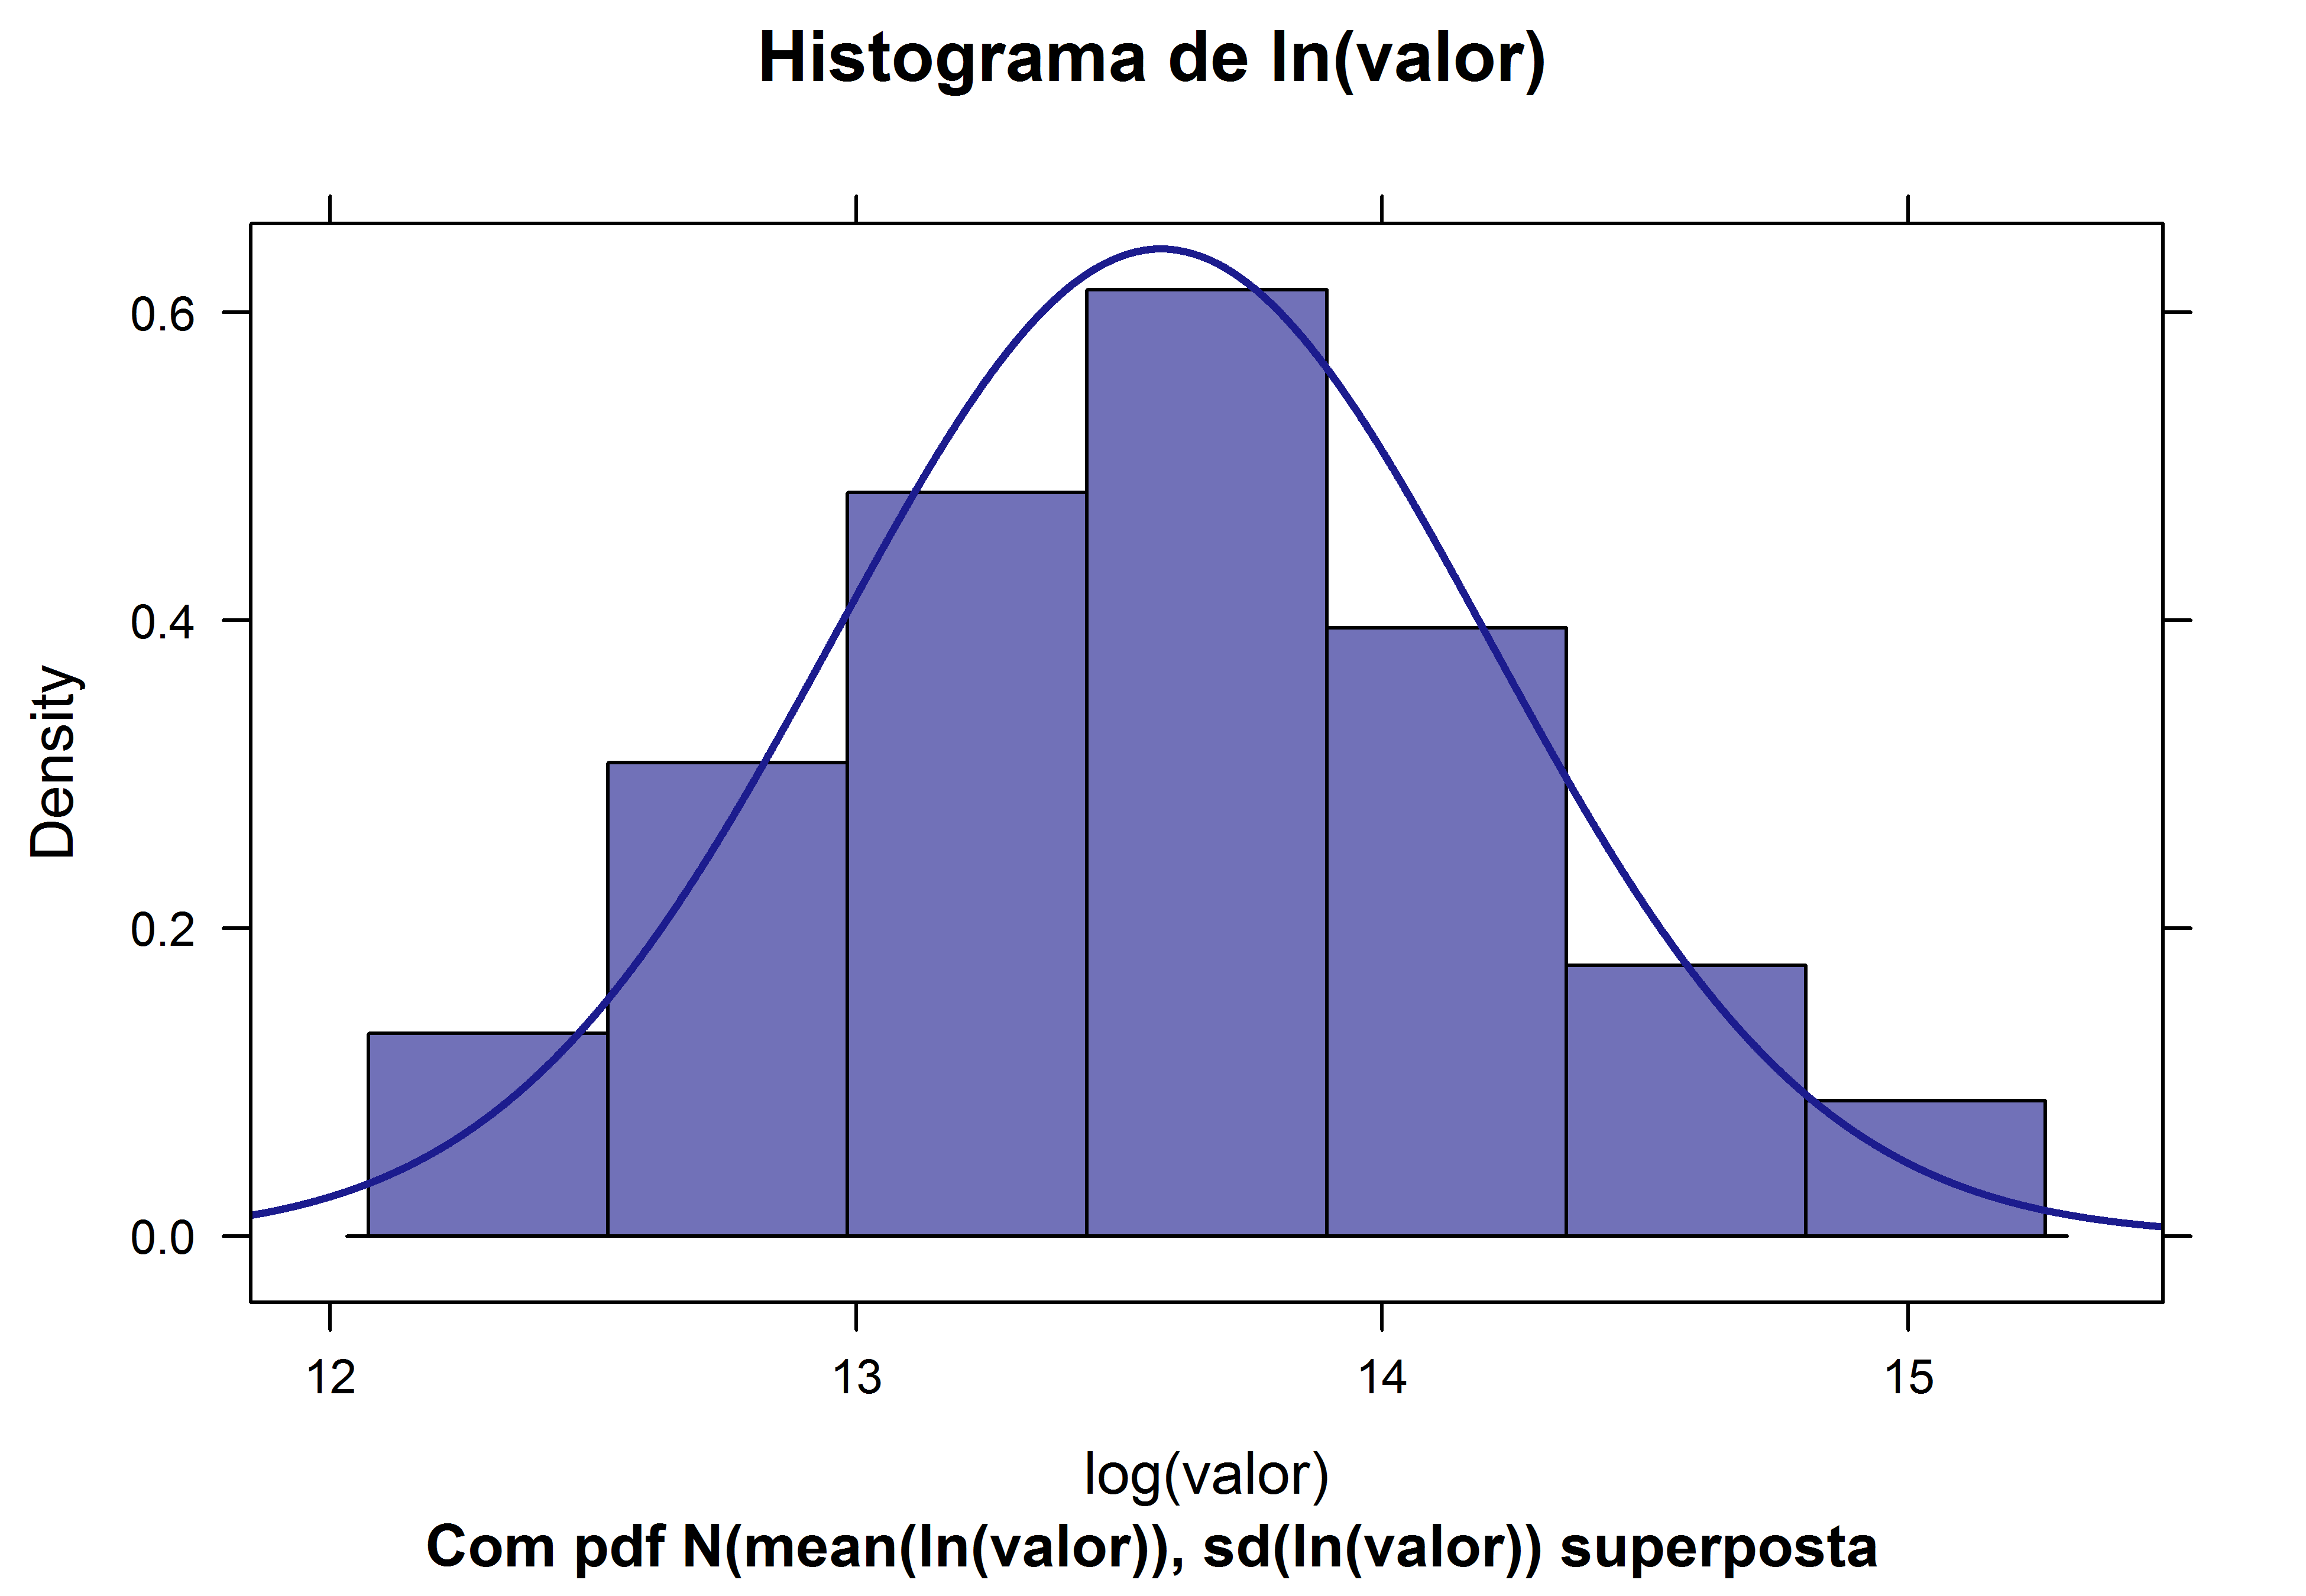
\includegraphics[width=0.7\linewidth]{images/hist_densidade2-1} 

}

\caption{Histograma com função densidade de probabilidade normal superposta}\label{fig:hist_densidade2}
\end{figure}

\subsection{Modelos}\label{modelos}

Detectando-se a presença de variável resposta com distribuição
lognormal, pode-se proceder da seguinte maneira:

\subsubsection{Modelo linear com a variável resposta
transformada}\label{modelo-linear-com-a-variavel-resposta-transformada}

É fácil mostrar que o modelo linear com a variável resposta
logaritmizada, ou seja, com distribuição normal, é melhor ajustado que o
modelo linear de uma variável resposta lognormal.

A função máxima verossimilhança de Box-Cox também vai apresentar como
transformação ótima a transformação logarítimica, como demonstra a
figura \ref{fig:boxcox}

\begin{figure}[H]

{\centering 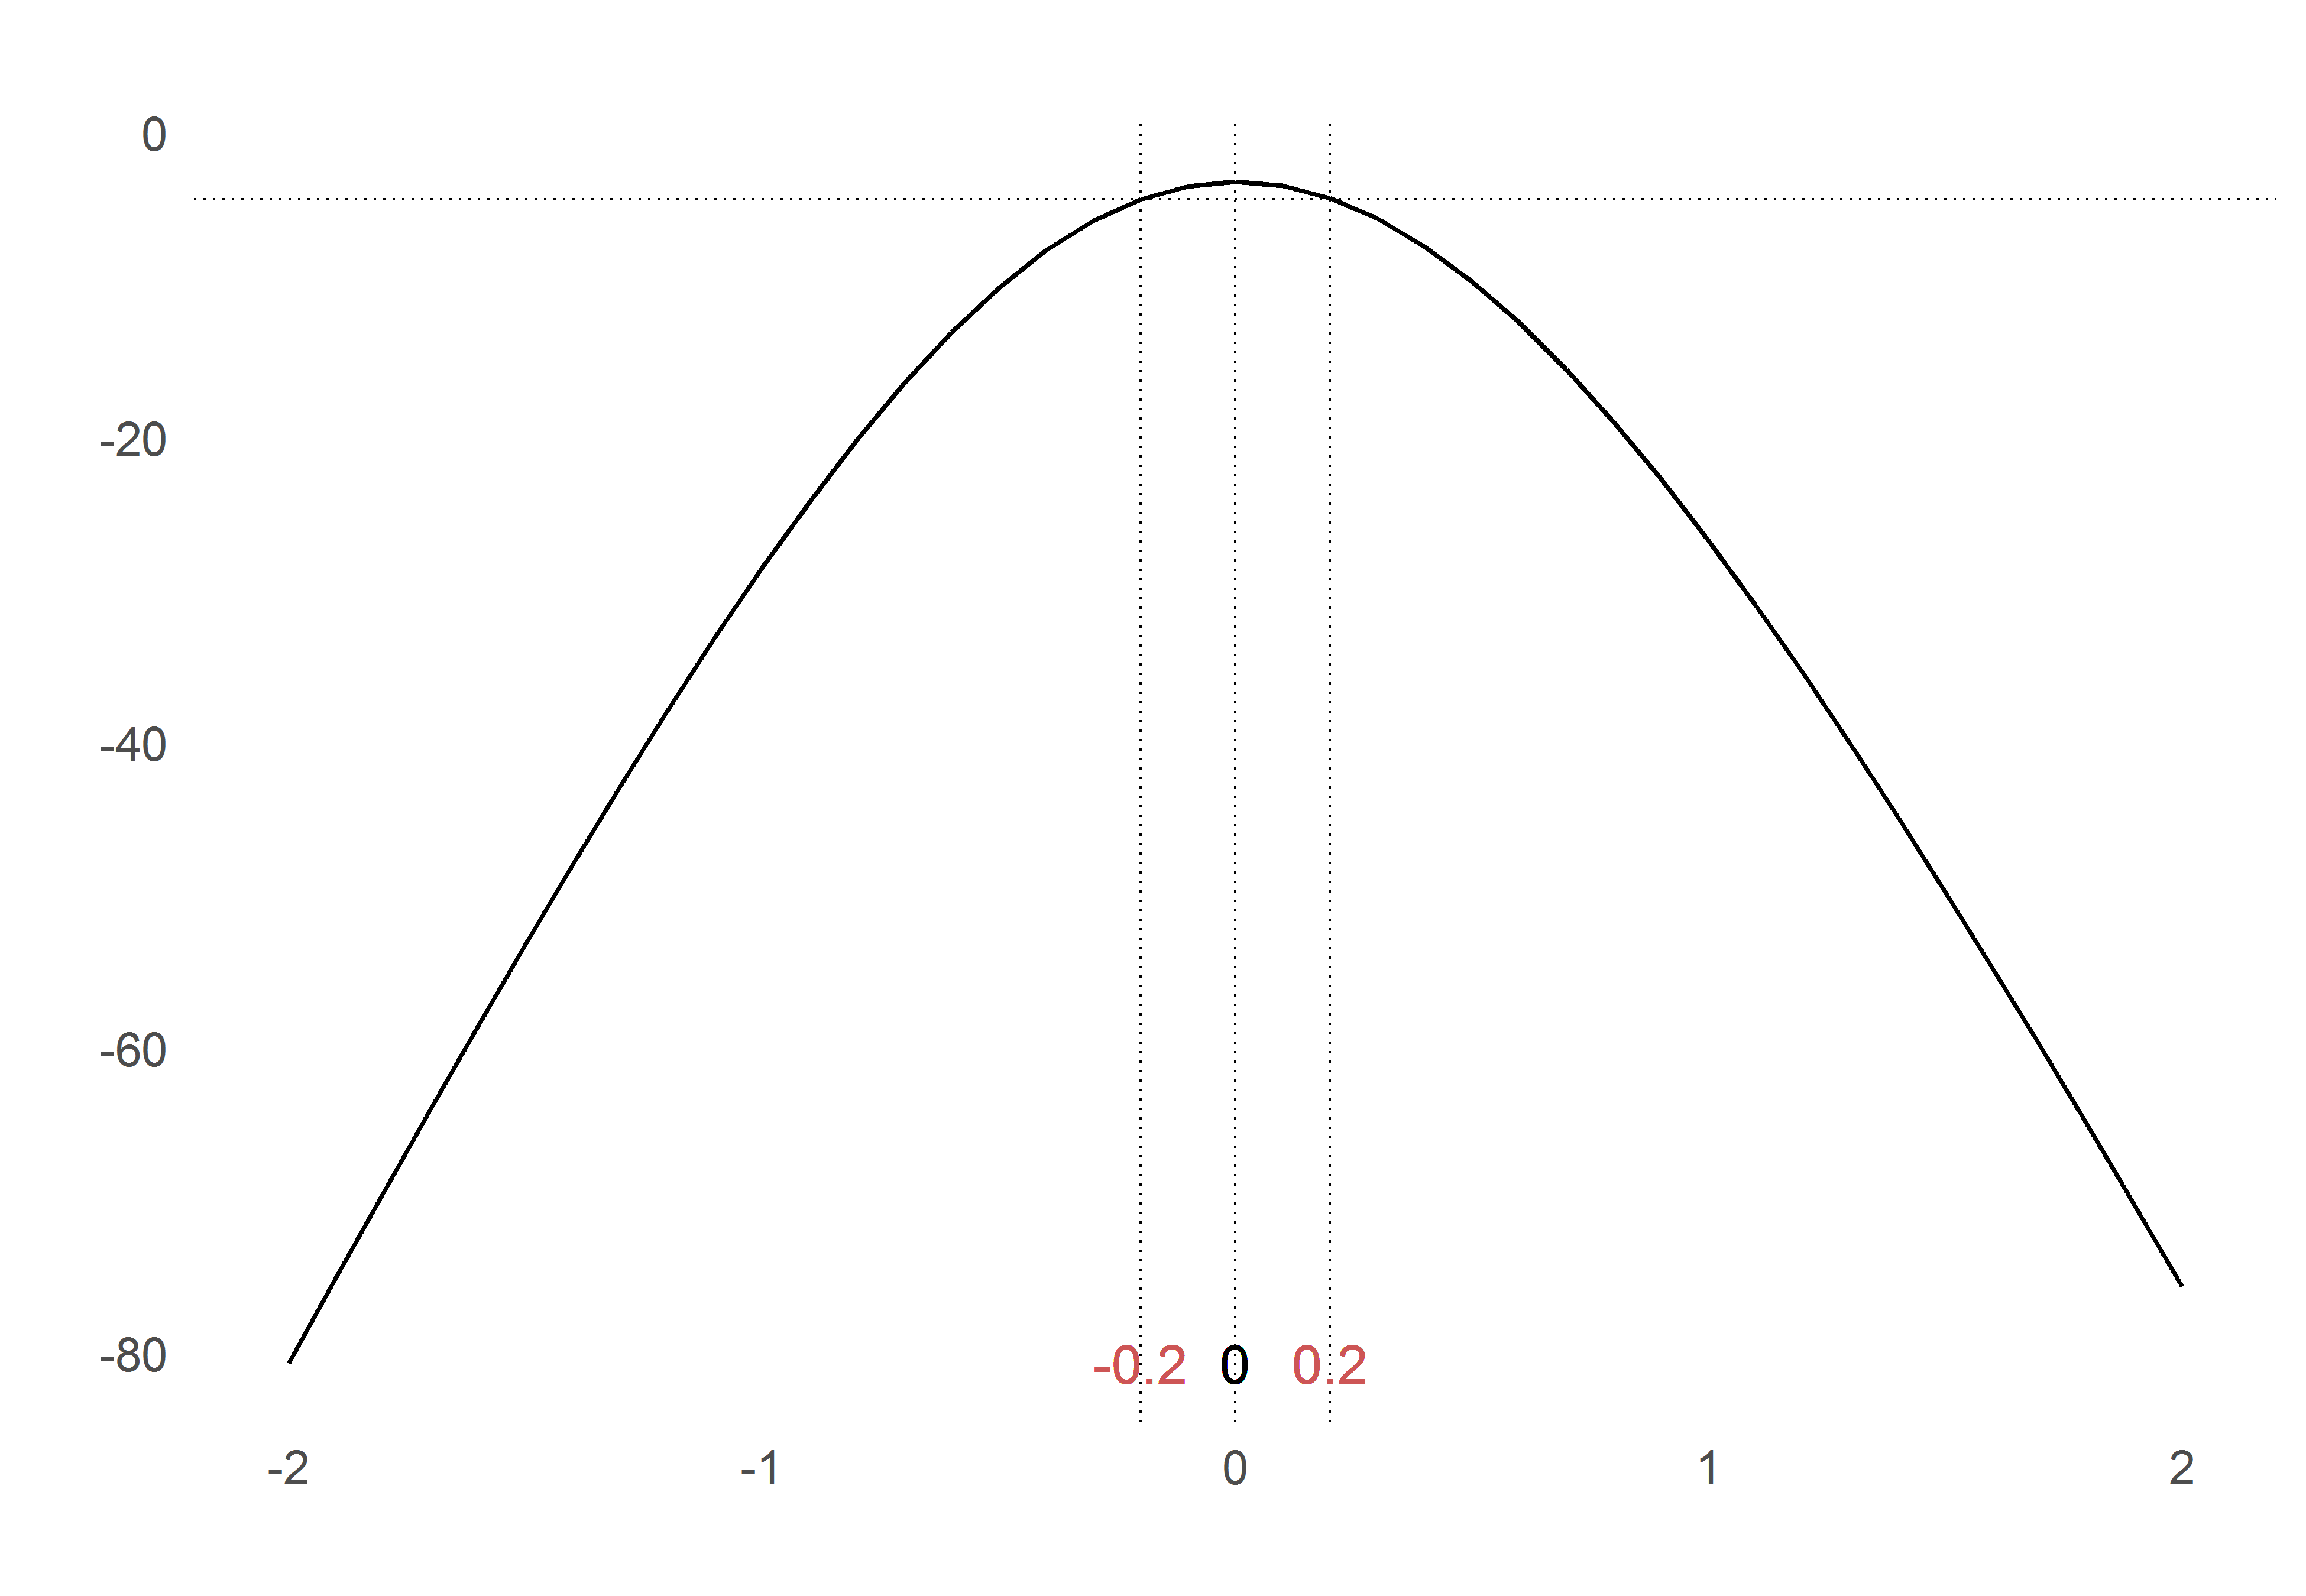
\includegraphics[width=0.7\linewidth]{images/boxcox-1} 

}

\caption{Gráfico da função verossimilhança de Box-Cox}\label{fig:boxcox}
\end{figure}

Na tabela \ref{tab:tabela} é possível comparar os modelos com e sem a
transformação da variável resposta, assim como o modelo de regressão de
poisson, que será visto na próxima seção.

\begin{table}[!htbp] \centering 
  \caption{Comparação entre modelos com e sem transformação da variável resposta} 
  \label{tab:tabela} 
\begin{tabular}{@{\extracolsep{5pt}}lcc} 
\\[-1.8ex]\hline 
\hline \\[-1.8ex] 
 & \multicolumn{2}{c}{\textit{Dependent variable:}} \\ 
\cline{2-3} 
\\[-1.8ex] & valor & log(valor) \\ 
\\[-1.8ex] & (1) & (2)\\ 
\hline \\[-1.8ex] 
 area\_total & 2,893.178 & 0.002 \\ 
  & (2,065.405, 3,720.951) & (0.001, 0.002) \\ 
  & t = 6.850 & t = 4.886 \\ 
  & p = 0.00000$^{***}$ & p = 0.00002$^{***}$ \\ 
  & & \\ 
 quartos & 73,524.375 & 0.169 \\ 
  & ($-$34,814.143, 181,862.894) & (0.084, 0.255) \\ 
  & t = 1.330 & t = 3.870 \\ 
  & p = 0.191 & p = 0.0004$^{***}$ \\ 
  & & \\ 
 suites & 111,000.591 & 0.088 \\ 
  & (8,045.131, 213,956.052) & (0.007, 0.170) \\ 
  & t = 2.113 & t = 2.121 \\ 
  & p = 0.041$^{**}$ & p = 0.040$^{**}$ \\ 
  & & \\ 
 garagens & 148,427.448 & 0.175 \\ 
  & (49,657.102, 247,197.795) & (0.097, 0.253) \\ 
  & t = 2.945 & t = 4.394 \\ 
  & p = 0.006$^{***}$ & p = 0.0001$^{***}$ \\ 
  & & \\ 
 dist\_b\_mar & $-$223.217 & $-$0.0003 \\ 
  & ($-$434.862, $-$11.571) & ($-$0.0004, $-$0.0001) \\ 
  & t = $-$2.067 & t = $-$3.215 \\ 
  & p = 0.045$^{**}$ & p = 0.003$^{***}$ \\ 
  & & \\ 
 padraomedio & $-$146,549.393 & 0.268 \\ 
  & ($-$354,850.457, 61,751.672) & (0.103, 0.433) \\ 
  & t = $-$1.379 & t = 3.190 \\ 
  & p = 0.176 & p = 0.003$^{***}$ \\ 
  & & \\ 
 padraoalto & $-$56,064.550 & 0.334 \\ 
  & ($-$264,003.525, 151,874.426) & (0.169, 0.498) \\ 
  & t = $-$0.528 & t = 3.975 \\ 
  & p = 0.600 & p = 0.0003$^{***}$ \\ 
  & & \\ 
 Constant & 33,953.788 & 12.315 \\ 
  & ($-$267,469.800, 335,377.375) & (12.076, 12.553) \\ 
  & t = 0.221 & t = 101.170 \\ 
  & p = 0.827 & p = 0.000$^{***}$ \\ 
  & & \\ 
\hline \\[-1.8ex] 
Observations & 50 & 50 \\ 
R$^{2}$ & 0.906 & 0.940 \\ 
Adjusted R$^{2}$ & 0.890 & 0.930 \\ 
Akaike Inf. Crit. & 1,375.659 & $-$29.275 \\ 
Residual Std. Error (df = 42) & 207,903.003 & 0.165 \\ 
F Statistic (df = 7; 42) & 57.731$^{***}$ & 94.063$^{***}$ \\ 
\hline 
\hline \\[-1.8ex] 
\textit{Note:}  & \multicolumn{2}{r}{$^{*}$p$<$0.1; $^{**}$p$<$0.05; $^{***}$p$<$0.01} \\ 
\end{tabular} 
\end{table}

\subsection{Retransformação de
variáveis}\label{retransformacao-de-variaveis}

O problema da transformação da variável resposta no logarítmo da
variável resposta original, é que devemos estudar como proceder na
retranformação da variável, para efetuar a avaliação do imóvel.

Para isto, utilizamos o valor esperado da variável log-normal, ou seja:

\[\mathbb{E}(X) = \exp(x + 0.5\sigma^2)\]

\section{CONCLUSÃO}\label{conclusao}

Foi possível demonstrar de maneira gráfica que os dados da variável
\texttt{valor} apresentados se ajustam bem a uma distribuição lognormal
equivalente. Por definição, então, o logaritmo da variável possui
distribuição normal.

0 valor mais provável para a variável resposta, então, é Valor Esperado
da variável. Logo, a retransformação da variável deve ser feita para a
média da variável log-normal.

\newpage

\hypertarget{anexo-i}{\section*{ANEXO I}\label{anexo-i}}
\addcontentsline{toc}{section}{ANEXO I}

\begin{table}[H]
\centering\rowcolors{2}{gray!6}{white}

\begin{tabular}{rrrrrrl}
\hiderowcolors
\toprule
valor & area\_total & quartos & suites & garagens & dist\_b\_mar & padrao\\
\midrule
\showrowcolors
1060000 & 350.00 & 3 & 1 & 2 & 720 & medio\\
510000 & 136.56 & 3 & 1 & 1 & 665 & medio\\
780000 & 164.77 & 3 & 1 & 2 & 415 & medio\\
550000 & 174.58 & 3 & 1 & 1 & 320 & medio\\
850000 & 123.01 & 3 & 1 & 3 & 895 & alto\\
\addlinespace
300000 & 89.83 & 2 & 0 & 1 & 645 & baixo\\
750000 & 174.00 & 2 & 1 & 2 & 860 & alto\\
650000 & 123.00 & 3 & 1 & 1 & 745 & alto\\
620000 & 121.00 & 3 & 1 & 1 & 745 & alto\\
740000 & 109.00 & 3 & 1 & 1 & 300 & medio\\
\addlinespace
770000 & 170.00 & 3 & 1 & 2 & 590 & medio\\
680000 & 141.00 & 3 & 1 & 1 & 290 & medio\\
850000 & 174.00 & 3 & 1 & 1 & 465 & medio\\
420000 & 105.00 & 3 & 1 & 0 & 60 & baixo\\
547000 & 128.00 & 3 & 1 & 1 & 745 & alto\\
\addlinespace
1600000 & 163.00 & 4 & 2 & 2 & 90 & alto\\
1320000 & 230.00 & 3 & 1 & 2 & 215 & alto\\
615000 & 108.00 & 3 & 1 & 1 & 745 & alto\\
705000 & 174.00 & 2 & 1 & 2 & 900 & alto\\
418000 & 85.00 & 1 & 0 & 1 & 620 & alto\\
\addlinespace
270000 & 71.00 & 2 & 0 & 0 & 1380 & baixo\\
418000 & 100.00 & 1 & 1 & 1 & 620 & alto\\
650000 & 90.00 & 2 & 1 & 1 & 215 & alto\\
700000 & 161.00 & 2 & 1 & 2 & 500 & alto\\
680000 & 174.00 & 2 & 1 & 2 & 860 & alto\\
\addlinespace
420000 & 76.00 & 2 & 1 & 1 & 700 & baixo\\
195000 & 48.00 & 1 & 0 & 0 & 730 & baixo\\
290000 & 66.00 & 1 & 0 & 1 & 745 & baixo\\
272000 & 50.00 & 1 & 0 & 1 & 1430 & baixo\\
430000 & 61.00 & 2 & 0 & 1 & 170 & baixo\\
\addlinespace
895000 & 109.00 & 3 & 1 & 1 & 530 & medio\\
450000 & 89.00 & 2 & 0 & 1 & 745 & medio\\
1950000 & 393.00 & 3 & 1 & 3 & 550 & alto\\
2150000 & 578.00 & 3 & 2 & 3 & 260 & alto\\
940000 & 182.00 & 3 & 1 & 2 & 200 & medio\\
\addlinespace
1400000 & 262.00 & 4 & 1 & 1 & 60 & alto\\
1090000 & 205.00 & 3 & 0 & 3 & 465 & medio\\
1272000 & 196.00 & 3 & 3 & 2 & 610 & alto\\
2800000 & 463.00 & 3 & 3 & 3 & 590 & alto\\
1796000 & 273.00 & 3 & 3 & 4 & 140 & medio\\
\addlinespace
1400000 & 330.00 & 4 & 2 & 2 & 655 & alto\\
3000000 & 533.00 & 4 & 3 & 4 & 427 & alto\\
1200000 & 221.00 & 3 & 3 & 2 & 607 & alto\\
800000 & 220.00 & 3 & 1 & 1 & 1000 & medio\\
950000 & 127.00 & 2 & 1 & 1 & 60 & medio\\
\addlinespace
2061000 & 362.00 & 3 & 3 & 4 & 310 & alto\\
1326000 & 315.00 & 3 & 3 & 3 & 600 & alto\\
850000 & 151.00 & 3 & 1 & 2 & 660 & medio\\
1650000 & 246.00 & 3 & 3 & 3 & 307 & alto\\
650000 & 159.72 & 3 & 1 & 1 & 120 & medio\\
\bottomrule
\end{tabular}
\rowcolors{2}{white}{white}
\end{table}

\section*{REFERÊNCIAS}\label{referencias}
\addcontentsline{toc}{section}{REFERÊNCIAS}

\hypertarget{refs}{}
\hypertarget{ref-portalaction}{}
ACTION, P. Distribuição log-normal.. Disponível em:
\textless{}\url{http://www.portalaction.com.br/probabilidades/615-distribuicao-log-normal}\textgreater{}..

\hypertarget{ref-fda}{}
FDA. \textbf{Guideline for the format and content of the clinical and
statistical sections of new drug applications}. Food and Drug
Administration, Public Health Service, US Department of Health and Human
Services, 1988.

\hypertarget{ref-hochheim}{}
HOCHHEIM, N. \textbf{Engenharia de avaliações - módulo básico}.
Florianópolis: IBAPE - SC, 2015.

\hypertarget{ref-keene}{}
KEENE, O. N. The log transformation is special. \textbf{Statistics in
Medicine}, v. 14, p. 811--819, 1985.


\end{document}
